%%%%%%%%%%%%%%%%%%%%%%%%%%%%%%%%%%%%%%%% 
% Masters This 
%
% Thesis template is based on templates by:
% - Mario Román (https://github.com/mroman42)
% - Steve Gunn (http://users.ecs.soton.ac.uk/srg/softwaretools/document/templates/)
% - Sunil Patel (http://www.sunilpatel.co.uk/thesis-template/)
% 
% Modifications done by Pedro Bonilla. 
% Template license:
% CC BY-NC-SA 3.0 (http://creativecommons.org/licenses/by-nc-sa/3.0/)
%
%%%%%%%%%%%%%%%%%%%%%%%%%%%%%%%%%%%%%%%%%

%----------------------------------------------------------------------------------------
%	PACKAGES AND OTHER DOCUMENT CONFIGURATIONS
%----------------------------------------------------------------------------------------

\documentclass[
11pt,
% oneside, % Two side (alternating margins) for binding by default, uncomment to switch to one side
english, % ngerman for German
singlespacing, % Single line spacing, alternatives: onehalfspacing or doublespacing
%draft, % Uncomment to enable draft mode (no pictures, no links, overfull hboxes indicated)
%nolistspacing, % If the document is onehalfspacing or doublespacing, uncomment this  to set spacing in lists to single
%liststotoc, % Uncomment to add the list of figures/tables/etc to the table of contents
%toctotoc, % Uncomment to add the main table of contents to the table of contents
%parskip, % Uncomment to add space between paragraphs
%nohyperref, % Uncomment to not load the hyperref package
headsepline, % Uncomment to get a line under the header
%chapterinoneline, % Uncomment to place the chapter title next to the number on one line
%consistentlayout, % Uncomment to change the layout of the declaration, abstract and acknowledgements pages to match the default layout
]{MastersDoctoralThesis} % The class file specifying the document structure


\usepackage[utf8]{inputenc} % Required for inputting international characters
\usepackage[T1]{fontenc} % Output font encoding for international characters
\usepackage{stmaryrd}
\usepackage{mathpazo} % Use the Palatino font by default
\usepackage[font=itshape]{quoting} 
\usepackage[toc,page]{appendix}
\usepackage{pdfpages}
\usepackage[backend=biber,style=numeric]{biblatex} 
\usepackage[activate={true,nocompatibility},final,tracking=true,kerning=true,spacing=true,factor=1100,stretch=10,shrink=10]{microtype}
\usepackage{eso-pic}
\usepackage[autostyle=true]{csquotes} 


\newenvironment{sproof}{\renewcommand{\proofname}{Sketch Proof}\proof}{\endproof}

\addbibresource{./example.bib} % The filename of the bibliography

\defbibcheck{uncited}{
  \ifciteseen
    {\skipentry}
    {}
}


% ----------------------------------------------------------------------------------
%	MARGIN SETTINGS
%----------------------------------------------------------------------------------

\geometry{
	paper=a4paper, % Change to letterpaper for US letter
	inner=2.5cm, % Inner margin
	outer=3.8cm, % Outer margin
	bindingoffset=.5cm, % Binding offset
	top=1.5cm, % Top margin
	bottom=1.5cm, % Bottom margin
	%showframe, % Uncomment to show how the type block is set on the page
}

%----------------------------------------------------------------------------------
%	THESIS INFORMATION AND METADATA
%----------------------------------------------------------------------------------
\usepackage[allcolors=myred]{hyperref}

\author{Pedro Bonilla Nadal}
\newcommand{\miTitulo}{Dependent Typing through Closed Cartesian Categories.\\\xspace}
\newcommand{\miNombre}{Pedro Bonilla Nadal\xspace} 
\newcommand{\miGrado}{Máster en Matemáticas y Aplicaciones}
\newcommand{\miFacultad}{Facultad de Ciencias}
\newcommand{\miUniversidad}{Universidad Autónoma de Madrid}
% Añadir tantos tutores como sea necesario separando cada uno de ellos
% mediante el comando `\\\medskip` y una línea en blanco
\newcommand{\miTutor}{
Dr. Ángel González Prieto  \\ \emph{Departamento de Matemáticas \\ Universidad Autónoma de Madrid}}
\newcommand{\miCurso}{2020-2021\xspace}
\newcommand{\misPalabrasClave}{HOTT, McLane}
\newcommand{\K}{\mathbb{K}}


\hypersetup{pdfinfo={
            Title={\miTitulo},
            Author={\miNombre},
            Director1={Dr. Ángel González Prieto},
            Ndirectores={1}
            Tipo={TFM},
            Curso={\miCurso},
            MSC={ MSC2020},
            Palabrasclave={\misPalabrasClave},
          }
        }

\AtBeginDocument{
\hypersetup{pdftitle=\miTitulo} 
\hypersetup{pdfauthor=\miNombre}
\hypersetup{pdfkeywords=\misPalabrasClave}
}

%%%%%%%%%%%%%%%%%%%%%%%%%%%%%%%%%%%%%%%%%%%%%%%%%%%%%%%%%%%%%%%%%%%%%%%%%%%%%%%%%%%


%----------------------------------------------------------------------------------
%          OTHER IMPORTS
%----------------------------------------------------------------------------------




\usepackage{titlesec}


%\usepackage[british]{babel}
\usepackage{caption}
\usepackage{adjustbox}
\usepackage{enumitem}
\usepackage{boldline}
\usepackage{amssymb, amsmath}
\usepackage{amsthm}
\usepackage{soul}
\usepackage{upgreek}
\usepackage{wrapfig}
\usepackage{mathtools}
\usepackage{epigraph}
\usepackage{algorithm}
\usepackage[noend]{algpseudocode}
\usepackage{soul}
\usepackage{graphicx}
\usepackage{mathrsfs}
\usepackage{xcolor}
\usepackage{listings}
\usepackage{tikz-cd}


\tikzcdset{arrow style=tikz, diagrams={>=stealth}}

\newtheorem{theorem}{Theorem}[section]
\newtheorem{corollary}{Corollary}[theorem]
\newtheorem{thesis}[theorem]{Thesis}
\newtheorem{lemma}[theorem]{Lemma}
\theoremstyle{definition}
\newtheorem{definition}{Definition}[section]
\newtheorem{proposition}{Proposition}[section]

\newtheorem{example}{Example}[section]
\newtheorem{remark}{Remark}[section]
\newcommand\myeq{\stackrel{\mathclap{\normalfont\mbox{?}}}{=}}

\newcommand{\R}{\mathbb{R}}
\newcommand{\N}{\mathbb{N}}
\newcommand{\dom}{\operatorname{dom}}
\newcommand{\colim}{\operatorname{colim}}
\newcommand{\codom}{\operatorname{codom}}
\newcommand{\hhom}{\operatorname{hom}}
\newcommand{\maybe}{\operatorname{Maybe}}
\newcommand{\oo}{\operatorname{ or }}
\newcommand{\ccase}{\operatorname{case}}
\newcommand{\iin}{\operatorname{in}}
\newcommand{\LL}{\mathcal{L}}
\newcommand{\QQ}{\mathbb{Q}}
\newcommand{\CC}{\mathcal{C}}
\newcommand{\MM}{\mathcal{M}}
\newcommand{\conv}{\operatorname{conv}}
\newcommand{\Int}{\operatorname{Int}}
\newcommand{\LC}{\lambda\operatorname{-Calc}}


\setlength\parindent{0pt}


\begin{document}
\frontmatter

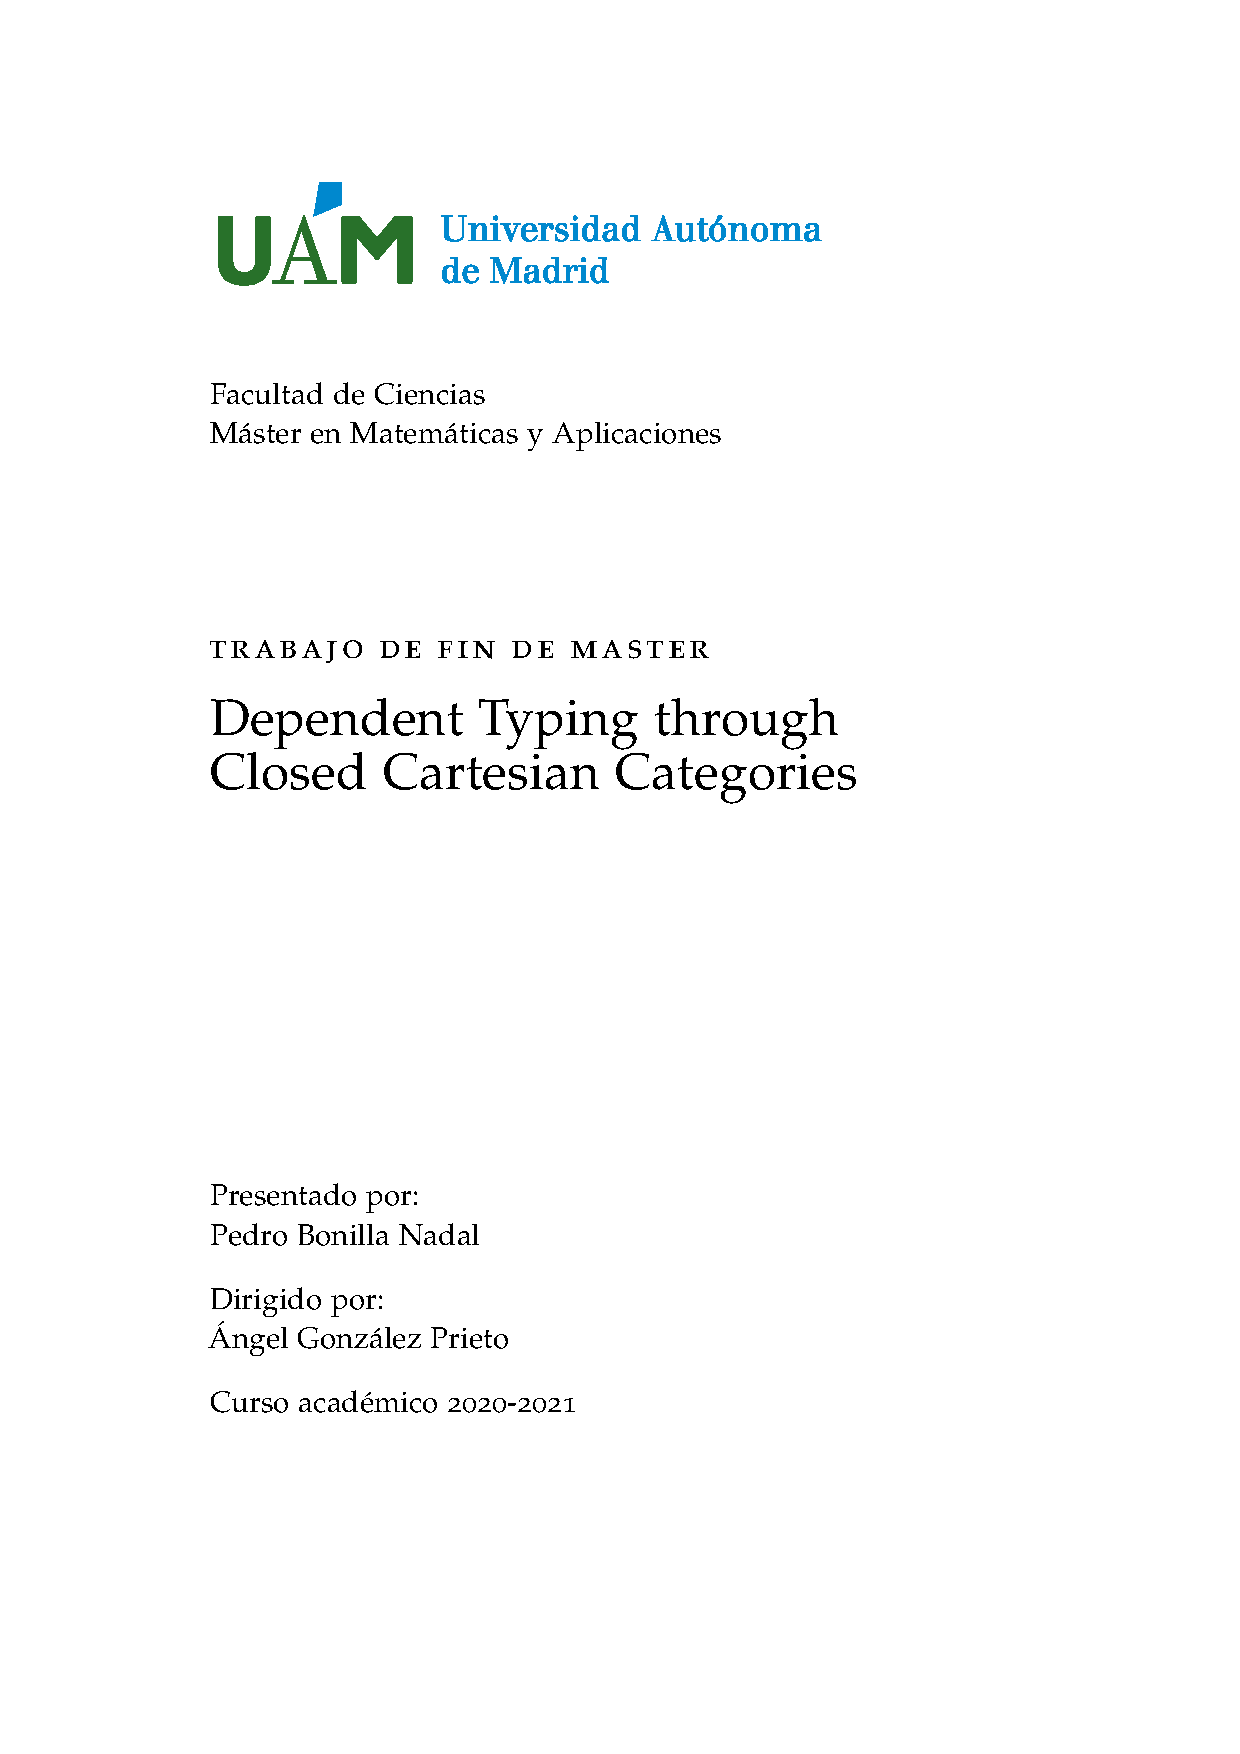
\includepdf{img/portada.pdf}
\cleardoublepage
% !TeX root = ../libro.tex
% !TeX encoding = utf8

%*******************************************************
% Little Dirty Titlepage
%*******************************************************

\thispagestyle{empty}

\begin{center}
  {\small TODO: incluir portada oficial}
  \large  

  \vspace*{\stretch{1}}

  \begingroup
  \huge{\miTitulo} \\
  {\small (Título provisional - busca uno definitivo - probablemente en mayo)}
  \bigskip
  
  \endgroup

  \textrm{\miNombre}

  \vspace{\stretch{5}}

\end{center}  

\newpage
\thispagestyle{empty}

\hfill

\vfill

\miNombre\ \textit{\miTitulo}.

Master's thesis.

Academic year \miCurso.\\

\begin{minipage}[t]{0.25\textwidth}
  \flushleft
  \textbf{Thesis\\ supervisor}
\end{minipage}
\begin{minipage}[t]{0.40\textwidth}
  \flushleft
  \miTutor
\end{minipage}
\begin{minipage}[t]{0.35\textwidth}
  \flushright
  \miGrado
  \medskip

  \miUniversidad
\end{minipage}
\begin{flushleft}
\end{flushleft}

\endinput

% !TeX root = ../libro.tex
% !TeX encoding = utf8
%
%*******************************************************
% Declaración de originalidad
%*******************************************************

\thispagestyle{empty}

\hfill\vfill

\textsc{Statement of Originality}\\\bigskip

D. \miNombre \\\medskip

 
I explicitly declare that the work presented as a Master's thesis (TFM) corresponding to the academic year \miCurso, is original, understood in the sense that it has not used sources for the elaboration of the work without citing them properly.

\medskip

Madrid, \today.
\begin{flushleft} 
Fdo: \miNombre 

\end{flushleft}

\vfill

\cleardoublepage
\endinput

% !TeX root = ../libro.tex
% !TeX encoding = utf8

%*******************************************************
% Dedication
%*******************************************************
\thispagestyle{empty}
\phantomsection 
\pdfbookmark[1]{Dedicatoria}{Dedicatoria}

\hfill
\vfill

\begin{flushright}
\itshape
Una dedicatoria a una persona probablemente.
\end{flushright}

\vfill

\cleardoublepage
\endinput

\pagestyle{thesis}
{
  \hypersetup{hidelinks}
  \setcounter{tocdepth}{2}
  \tableofcontents
}

%*******************************************************
% Introducción
%*******************************************************

% \manualmark
% \markboth{\textsc{Introducción}}{\textsc{Introducción}} 
\chapter{Introduction}

\section*{Main goals and results achieved}



\endinput
               
\begin{otherlanguage}{spanish}
  %*******************************************************
% Summary
%*******************************************************

\newpage



\chapter*{Summary}
\addcontentsline{toc}{chapter}{Summary}
\section*{Brief Summary}

English Abstract

\textbf{keywords:} 



\selectlanguage{spanish}
\section*{Resumen Extendido}

Resumen extendido en español

\textbf{palabras clave:} 


\selectlanguage{english}


% \endinput
                    
\end{otherlanguage}

\mainmatter
\part{Category Theory}
\thispagestyle{empty}
\label{Part1}





\chapter{First Notions of Category Theory}
\thispagestyle{empty}
%%%%%%%%%%%%%%%%%%%%%%%%%%%%%%%%%%%%%%%%%%%%%%%%%%%%%%%%%%%%%%%%%%%%%%%% 
\epigraph{“The human mind has never invented a labor-saving machine equal to algebra.” }{\textit{Stephan Banach (1925)}}

For us Category Theory is an area of interest on its own rights, rather than merely an elegant tool. Thus, we will introduce this theory with a point of view that emphasize the intuitive ideas behind each notion.\\

With this objective in mind, we will get into the habit of introducing the first examples even before introducing the formal definitions. Thus, when the formal definition is introduced it becomes meaningful.\\

The fundamental idea of Category Theory is that many properties can be unified if expressed in arrow diagrams. Intuitively, a diagram is a directed graph, such that each way of going from a node to another are equals. For example, the diagram:

\[
  \begin{tikzcd}
    & b \arrow[rd, "g"]& \\
    a\arrow[ru, "f"] \arrow[rr, "h", dashed] && c
  \end{tikzcd}
\]
Means that $f\circ g = h$. This approach to mathematics emphasises  at the relationships between elements, rather than at the structure of the elements themselves. In general, dashed lines means that the existence of that particular arrow is uniquely determined by the solid arrow presents in the diagram.\\

In this first chapter we introduce the notion of category and some useful properties. The principal references for this chapter are \cite{mac2013categories} and \cite{riehl2017category}. To show how categories can be used for programming we will illustrate several concepts with the programming language Haskell. Haskell references can be checked in \cite{milewski2018category}.

\section{Metacategories}
We will start by defining a concept independent of the set theory axioms: the concept of \emph{metacategory}. Then, categories will arise from studying these concepts within set theory. We follow  \cite{mac2013categories} for these definitions.\\


Traditionally, mathematics is based on the set theory. When we start set theory it is not necessary (it is not possible) to define what a set is. It is similar with the concepts of element and belonging, which are basic to set theory. Category theory can also be used to found mathematics. This theory provide meaning based on other concepts such as object, arrow or composition rather than sets or belonging. \\

\begin{definition} \label{def:metagraph}
  A \emph{metagraph} consist of \emph{objects}: $a,b,c..$ and \emph{arrows} $f,g,h...$. There are also two pairings: $\dom$ and $\codom$. This pairings assigns each arrow with an object. An arrow $f$ with $\dom(f)=a$ and $\codom(f)=b$ is usually denoted as $f:a\to b$.\\
\end{definition}

\begin{definition}
  A metacategory  is a metagraph with two additional operations and two properties:
  \begin{itemize}
  \item Operations:
    \begin{itemize}
      
    \item \emph{Identity}: assigns to each object $a$ an arrow $1_a:a\to a$. 
    \item \emph{Composition}: assigns to each pair of arrows $f,g$ with $\codom(f)=\dom(g)$ and arrow $g\circ f$ such that the diagram:

      \[
        \begin{tikzcd}
          & b \arrow[rd, "g"]& \\
          a\arrow[ru, "f"] \arrow[rr, "g\circ f",swap, dashed] && c
        \end{tikzcd}
      \]

      commutes. The arrow $g\circ f$ is called the \emph{composite} of $f$  and $g$.
    \end{itemize}

  \item Properties:
    \begin{itemize}
    \item \emph{Associative}: given arrows $f,g,h$, we have that,
      $$(g\circ f) \circ h = g \circ (f \circ h).$$
    \item \emph{Unit}: given an object $a$, and arrows $f,g$ such that $\dom (f)= a$ and $\codom (g) = a$, we have that,
      $$1_a \circ g = g, \qquad f \circ 1_a = f.$$
    \end{itemize}
  \end{itemize}
  In the context of categories and metacategories, arrows are often called \emph{morphisms}.
\end{definition}

We have just define what a  metacategory is without any need of set and elements. In most cases we will rely in a set theory interpretation of this definitions, as most examples (specially with our interest in computational example) will rely on this theory. Nonetheless, whenever possible, we will define the concepts working only in terms of objects and arrows.\\



% Diagramas de existencia condicionada.!!
% We will also need diagrams that represents the existence of arrows due to the existence other arrows. , given objects $a,b,c$ and arrows $d$



\section{Set theory categories}
Despite being an alternative foundation of mathematics, in general we will work with categories interpreted with notions of set theory. Unless otherwise stated, we will use the Zermelo-Fraenkel-Gödel axiomatics with Axiom of Choice. In this we are going to difference between \emph{small sets} and \emph{classes}. Sets that are not small are called \emph{large sets}. We recommend \cite{kunen2014set} for more information.\\

We have no interest in this work in the reformulation of axioms. Note that  we have defined a meta-category without the need for notions of sets. In the same way,  many definitions and propositions relating to this theory can be considered without the need for notions of sets.\\


From now on, we will work based on set theory. Despite that, it is useful to take into account that most of the concept here presented can be defined without making use of this Theory. 

\begin{definition}
  A category (resp. graph) is an interpretation of a metacategory (resp. metagraph) within a set theory.
\end{definition}


\footnote{{\color{black} There is a discussion here that must be addressed at the end}}That is, a graph/category is a pair $(O,A)$ where a collection $O$ consisting of all objects as well as a collection $A$ consisting of all arrows. Their elements hold the same properties that objects and arrows hold on metacategories / metagraph.\\


We will focus on the category. First, we define the function homeset of a category $C=(O,A)$, wrote as $\hhom_{C}$, as the function:
\begin{align*}
  && \hhom_{C}: O \times O &\mapsto \mathcal{P}(A)&\\
  \displaystyle &\ &(a,b)&\mapsto \{f\in A | f:a\to b\}&
\end{align*}

We will refer to the collection of objects of a category $C$ as $Ob(C)$ and the collection of arrows as $Ar(C)$. When there is no possibility of confusion we will state $c\in C$ meaning either $c\in Ob(C)$ or $c\in Ar(C)$.

\begin{definition}
  We say that a category is \emph{small} if the collection of objects is given by a set (instead of a proper class). We say that a category is \emph{locally small} if every homesets is a set.
\end{definition}

We proceed to introduce a comprehensive list of examples, so that it is already introduced in subsequent chapters. 
\begin{example}

  \begin{itemize}  \ 
  \item The elementary categories:
    \begin{itemize}
    \item The category $0 = ( \emptyset, \emptyset)$ where every property of metacategories is trivially satisfied.
    \item The category $1 = (\{e\},\{1_e\})$.
    \item The category $2 = (\{a,b\},\{1_a,1_b,f:a\to b\})$\label{2-category}
    \end{itemize}

  \item Discrete categories: are categories where every arrow is an identity arrow. This are sets regarded as categories, in the following sense: every discrete category $C=(A, \{1_a : a \in A\})$ is fully identified by its set of object.  
  \item Monoids and Groups: A monoid is a category with one object (regarding the monoid of the arrows). In the same way, if we requires the arrows to be invertible, we can see a group as a single-object category. 
  \item Preorder: From a preorder $(A, \le)$ we can define a category $C = (A, B)$ where $B$ has an arrow $e: a \to b$ for every $a,b\in A$ such that $a \le B$. The identity arrow is the arrow that arise from the reflexive property of the preorders. 

  \item Large categories: these categories have a large set of objects. For example:
    \begin{itemize}
    \item The category $Top$ that has as objects all small topological spaces and as arrow continuous mappings.
    \item The category $Set$ that has as objects all small sets and as arrows all functions between them. We can also consider the category $Set_*$ of pointed small sets (sets with a distinguish point), and functions between them that maps preserving the marked point. This category, when restricted to finite sets, is known as $FinSet$.
    \item The category $Vect$ That has as object all small vector spaces and as arrows all the linear functions.
    \item The category $Grp$ that has as object all small vector group and as arrows all the homomorphism.
    \item The category $Top_*$ that has as object all small topological spaces with a distinguished point, and as arrows all the continuous functions that maps each distinguished points into distinguished points. Similarly we can consider $Set_*$ or $Grp_*$.
    \item The category $Grph$ that has as objects all small graphs, and as arrows all graphs morphisms.
    \end{itemize}

  \item The category $Hask$ of all Haskell types and all possible functions between two types.\\
    
  \end{itemize}
  Note that, for example, as natural numbers can be seen as either a set or a preorder, they also can be seen as a discrete category or a preorder category.
\end{example}


Simple enough categories can be easily described with graphs: there are as many objects as nodes in the diagram and an arrow in the category for each:
\begin{itemize}
\item Arrow in the graph. 
\item Composition of existing arrows.
\item Every node (identity arrow usually omitted in diagrams).
\end{itemize}

For example, we can fully represent the $2$ category with the diagram:

\[
  \begin{tikzcd}
    a\arrow[rr, "g"] && c\\
  \end{tikzcd}
\]




\subsection{Properties}

We can see that is common in mathematics to have an object of study (propositional logic clauses, groups, Banach spaces or types in Haskell). Once the purpose of studying these particular sets of objects is fixed, it is also common to proceed to consider the transformations between these objects (partial truth assignments, homomorphisms, linear bounded functionals or  functions in Haskell).\\

In categories, we have a kind of different approach to the subject. Instead of focusing on the objects themselves, we focus on how do they relate to each other. That is, we focus on the study of the arrows and how they composes. Therefore we can consider equal two objects that has the same relations with other objects. This inspire the next definition:

\begin{definition}\cite[Definition 1.1.9]{riehl2017category}
  Given a category $C=(O,A)$, a morphism $f: a \to b \in A$ is said to have a \emph{left inverse} (resp. \emph{right inverse}) if there exists a $g: b \to a \in A$ such that morphism $g \circ f = 1_b$ (resp. $f \circ g = 1_a$). A morpishm is an \emph{isomorphism} if it has both left and right inverse, sloppily called the \emph{inverse}. Two object are isomorphic is there exists an isomorphism between them.
\end{definition}


Is easy to follow that if a morphism has a left and a right inverse, they must be the same, thus implying the uniqueness of the inverse. Also one can see that this functions define, by precomposition, bijections between $\hhom(a,c)$ and $\hhom(b,c)$ for all $c\in O$.\\

We will now proceed to talk about certain arrows and objects that have properties that distinguish them from others.  The most useful example to gain an intuition of these properties is that of the $FinSet$ category, of all finite sets and functions between them.  Considering special arrows:\\

\begin{definition} An arrow $f$ is  \emph{monic} (resp. \emph{epic}) if it is \emph{left-cancelable} (resp. \emph{right-cancelable}), i.e.  $f\circ g = f \circ h \implies g = h$ (resp. $g\circ f = h \circ f \implies g = h$).
\end{definition}



In $FinSet$ these arrows are the injective functions (resp. surjective). Considering special objects:

\begin{definition}
  an object $a$ is \emph{terminal} (resp. \emph{initial}) if for every object $b$ there exists an unique arrow $f:b\to a$ (resp. $f:a\to b$).  An object that is both terminal and initial is called \emph{zero}.
\end{definition}

In $FinSet$ the initial object is the  empty set and the terminal object the one point set.

\begin{proposition}\label{terminal-proposition}
  Every two terminal object are isomorphic.
\end{proposition}
\begin{proof}
  Every terminal object has only one arrow from itself to itself, and necessarily this arrow has to be the identity. Let $a, b$ be terminal object and $f:a\to b$ and $g:b\to a$ be the only arrows with that domain and codomain. Then $f\circ g : a \to a \implies f \circ g = 1_a$. Analogously $g \circ f = 1_b$.\\
\end{proof}

% \subsubsection{Duality}
Another important property is the \emph{duality property}. This property tell us that for every theorem that we prove for categories, there exist another theorem that is automatically also true, by inverting the direction of the arrows. To formalize this idea, we define the concept of \emph{opposite category}.


\begin{definition}\cite[Definition 1.2.1]{riehl2017category}
  Let $C$ be any category. The opposite category $C^{op}$ has:
  \begin{itemize}
  \item the same objects as $C$,
  \item an arrow $f^{op}:b \to a\in C^{op}$ for each arrow $f: a\to b \in C$, so that the domain of $f^{op}$ is defined as the codomain of $f$ and viceversa.
  \end{itemize}
  The remaining structure of the category $C^{op}$ is given as follows:
  \begin{itemize}
  \item For each object $a$, the arrow $1_a^{op}$ serves as its identity in $C^{op}$.
  \item We observe that $f^{op}$ and $g^{op}$ are composable when $f$ and $g$ are, and define $f^{op} \circ g^{op} = (g \circ f)^{op}$.
  \end{itemize}
\end{definition}


The intuition is that we have the same category, only that all arrows are turned around. We can see that  for each theorem $T$ that we prove, we have reinterpretation that theorem to the opposite category. Intuitively this theorem is an equal theorem in which all the arrows have been turned around. For example: the proposition
\ref{terminal-proposition} can be reworked as:

\begin{proposition}\label{prop:initial}
  Every two initial object are isomorphic.
\end{proposition}


That is because being initial is the dual property of being terminal, that is, if $a\in C$ is a terminal object then $a\in C^{op}$ is an initial object. The property ``being isomorphic'' is its own dual.

\subsection{Transformation in categories}




% \subsubsection{Functors}
One of the main ways of defining a category is considering as object every small set with an structure (e.g. groups, monoids, vector spaces), and as morphism all functions that preserve structure. Then, we may also follow our study defining the structure preserving transformation of categories.

\begin{definition}
  Given two categories $C, B$, a \emph{functor} $F: B \to C$ is a pair of functions $F=(F':Ob(C)\to Ob(B),F'':Ar(C)\to Ar(B))$ (the \emph{object functor} and the \emph{arrow functor} respectively) in such a way that:
  $$F''(1_c) = 1_{F'c}, \ \forall c \in Ob(C), \qquad F''(f\circ g) = F''f \circ F''g, \ \ \forall f:a\to b,g: b\to c  \in Ar(C).$$

\end{definition}


Roughly speaking,  a functor is a morphism of categories. When there is no ambiguity we will represent both $F'$ and $F''$ with a single symbol $F$ acting on both objects and arrows. Also, it can be seen in the definition that whenever possible the parentheses of the functor will be dropped. This loss of parentheses will be replicated throughout the text, whenever possible.\\



\begin{remark}
  A functor $F$ can be defined only pointing out how it maps arrows, as how $F$ maps object can be defined with how it map identity arrows.
\end{remark}
Lets provide some examples of functors:\\



\begin{example}\ 
  \begin{itemize}
  \item {Forgetfull functor}: We have a variety of categories consisting of structures with sets as objects and functions that hold structure such as arrows (eg Top, Grp or Vect).\\
    
    Let $C$ one of such  categories, then we have a functor $F:C\to Set$ that maps each object to its underlying set and each arrow to the equivalent arrow between sets. That is, this functor forgets about the structure that is present in $C$.\\

    Additionally, we will often have functors defined $F:C\to Set$. For some cases of $C$ it also happen that the image of $Ob(C)$ by $F'$ has some more structure on it. In that case we will say that $F$ is an enriched functor for that cases.\\

    Another similar case of Forgetful functor is $\mathcal{U}:Cart \to Grph$ that maps each (small) category to their \emph{underlying} graph. 
  \item Fundamental group: In the context of algebraic topology we have the functor of the fundamental group $\Pi_1: Top_* \to Grp$. The most famous property of this function is that

    
   \begin{displayquote}
      ``Given continuous application $ f,g:X \to Y$ between two topological spaces induces an application of the group of loops of $X$ on the group of loops of $Y$ such that $\Pi_1(f \circ g) = \Pi_1(f) \circ \Pi_1(g)$.''
   \end{displayquote}

    that is, the functoriality of the function (taking also into account the fact that the identity of topological spaces is mapped to the identity of group). 

  \item Stone-\v{C}ech compactification\label{example:stone-cech}:  From the realm of functional análisis we have the following theorem:

    \begin{theorem} Let $\mathbb{K}=\mathbb R $ or $\mathbb C$ and let $\Omega$ be a completely regular Hausdorff topological space. Then there exists a compact Hausdorff topological space $\beta \Omega$ and a homeomorphism $\Phi$, from $\Omega$ to a dense subset of $\beta\Omega$. Moreover, for every continuous and bounded function $f: \Omega \to K$ there exists a unique $\overline{f} \in C(\beta \Omega)$ such that $\overline{f}\circ \Phi = f$ and the application $f \to \overline{f}$ is an isomorphism. Finally, $\beta \Omega$ is uniquely determined up to isomorphism by the above properties.
    \end{theorem}

    \begin{proof}
      We define the functional $\Delta: \Omega \to \Omega^{**}$   such that $\Delta(t)=\delta_t$ where $\delta_t(f) = f(t)$ is Dirac's operator .  It is enough to take as $\beta \Omega$ the closure of $\Delta(\Omega)$ in the induced weak-topology $\omega^*$ of $\Omega$ (since in the weak topology we have that a bounded closed is compact).  
      
      Given a continuous and bounded function $f:\Omega \to\mathbb K$ we can define the function $\overline{f}$ by injection of $\Omega$ and then limit to maintain continuity (which will exist by compactness and boundedness of $f$). Thus the maximum of $\overline{f}$ can be reached by a sequence of points injected from  $\Omega$ obtaining that   
      $${\displaystyle\max\left\{|\ \overline{f}\ (s)\ | : s \in \beta\Omega\right\} = \sup\left\{| f(s) |: s \in \Omega\right\}}.$$
      
      The application $f \mapsto \overline{f}$ is therefore an isometric isomorphism. Thanks to this isometric isomorphism the function spaces and by the Banach-Stone theorem\cite[Theorem 3]{banach1932theorie} we have uniqueness up to isomorphisms. 
    \end{proof}

    Based on this theorem we can define a functor  $\beta:Hauss \to Comp$ where $Hauss$ is the category of Completely regular Haussdorff  Spaces and continuous functions, and $Comp$ the category of Compact Haussdorff Spaces along with continuous function. This functor:
    \begin{itemize}
    \item Take an object $\Omega \in Hauss$ to $\beta(\Omega) = \beta\Omega$:
    \item Take an arrow $f:\Omega \to \Omega'\in Hauss$ to $\Delta(f)$ and the complete it by continuity as in the previous proof.
    \end{itemize}
    
    % {\color{red} Question}: I want to include this example of functor in order to later reuse it in universality section (opening of chapter 2).\\

    % I'm having a bit of trouble doing this though, as I do not see how does it maps arrows. I have found this proof of its functoriality:

    % \begin{displayquote}
    %   As is usual for universal constructions like this, the extension property makes $\Beta$ a functor from $Top$ (the category of topological spaces) to $CHaus$ (the category of compact Hausdorff spaces).
    % \end{displayquote}

    % However, I was hoping to provide a more elemental proof, so I will continue looking. If nothing is founded, there will be no problem to drop this example, or to explain directly when extension property is explained.
    % {\color{red} End Question}


  \item Group actions:\label{group-action} Every group action can be seen as a functor from a Group to a Set.\\
    
    Let $G$ be a group seen as a category with only one element and $X$ be a set seen as a discrete category. Then, an action is a representation of the group of the endomorphism of the set, that is, an action $\alpha$ associate each element of the group with an function $\alpha(g):X\to X$ such that the product of element of the group is maintain via composition. That is for $g\in Ar(G)$ we have that $\alpha(g) \in Ar(X)$  and for all $ g,f\in Ar(G):$
    $$\alpha(g\circ f) = \alpha(g) \circ \alpha(f).$$

    Notice that, by the definition of $G$, the composition $g\circ f$ actually correspond to the product in $G$.
    
    Note that is a group seen as a category the product is the composition thus having the functoriality.\\
    
  \item \texttt{Maybe} Method in Haskell \cite[Section 7.1]{milewski2018category}: In Haskell the definition of Maybe is a mapping from a type $a$ to a type $\maybe  a$. We define the BN notation used in the example in \ref{def:BN-Notation}.

    \begin{center}
      \begin{lstlisting}[language=Haskell,caption={Declaration of Maybe},captionpos=b]
        data Maybe a = Nothing | Just a
      \end{lstlisting}
    \end{center}
    
    Note that \texttt{Maybe a} is not a type but a function of types. In order for it to be an endofunctor of the $Hask$ category we will need for it to also map function. Let $f: a \to b\in Hask$, then we define the function
    $$\maybe  f: \maybe a \to \maybe b$$
    such that
    $$(\maybe  f) (Nothing) = Nothing, \qquad (\maybe f) (Just\  a) = Just\  f(a).$$
    Note that $(\maybe id_a) (\maybe a) = Nothing\  |\  Just\  id_a(a) =  \maybe a$.
  \end{itemize}
\end{example}


We can now construct the category of all small categories $Cat$. This category has as object all small categories and as arrows all functor between them. Note that $Cat$ does not contain itself, since it is a large category.\\

We can consider some properties in functors. Note that we can consider a functor $T:C\to D$ as a set function over homeset, that is, a function: 
$$T:\hhom_C(a,b) \to \{Tf: Ta \to Tb | f \in C\} \subset \hhom_D(Ta,Tb)$$

\begin{definition}
  A functor $T:C\to D$ is \emph{full} if it is surjective as a function over homesets, i.e. if the function $T:\hhom_C(a,b) \to  \hhom_D(Ta,Tb)$  is surjective for every $a,b \in C$. A functor is \emph{faithfull} if it is injective over homesets.
\end{definition}

As we have defined the concept of opposite category, we can consider functors $T:C^{op} \to D$. It is customary to refer to this type of functions a \emph{contravariant} functor from $C$ to $D$ and regular functors $F:C\to D$ as \emph{covariant}.




% \subsubsection{Natural Transformations}

We shall continue defining natural transformation. In the words of Saunders Mac Lane:

\begin{displayquote}
  ``Category has been defined in order to define functor and functor has been defined in order to define natural transformation.''
\end{displayquote}




One can see a functor $T:C\to D$ as a representation of a category in another, in the sense that a functor provide a picture of the category $C$ in $D$. Further into this idea, we can consider how to transform these drawings into each other. 

\begin{definition}
  Given two functor $T,S:C\to D$, a \emph{natural transformation} $\tau : T \Rightarrow S$ is a function from $Ob(C)$ to $Ar(D)$ such that for every arrow $f:c \to c' \in C$ the following diagram commutes:
  \[
    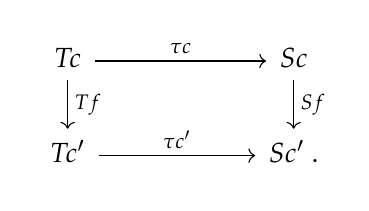
\begin{tikzpicture}
      \node {\begin{tikzcd}[column sep=20mm]
          Tc\ar[r,"\tau c"]\ar[d,"Tf"] & Sc\ar[d,"Sf"]\\
          Tc'\ar[r,"\tau c'"] & Sc'\ .
        \end{tikzcd}};
    \end{tikzpicture}
  \]

 A natural transformation where every arrow $\tau c$ is invertible is called a \emph{natural equivalence} and the functors are \emph{naturally isomorphic}.
\end{definition}
\begin{remark}
  In come context, subindex $\tau_c$ are used to note natural transformation, specially when working in composition with other arrows.
\end{remark}

That is a natural transformation is a map from pictures of $C$ in to pictures of $D$. Note that a natural transformation acts only on the domain of objects. Lets provide some examples.\\

When we have to define natural transformations  it will often be useful to define each arrow individually. In this case, with the same notation as in the definition,  we will note $\tau c = \tau_c: Tc \to Sc$. 

\begin{example}\ 
  \begin{itemize}
  \item The opposite group: We can define the opposite functor $(\cdot)^{op}: Grp \to Grp$ that maps $(G, *)$ to $(G; *^{op})$ where $a*^{op}b= b*a$ and maps a morphism $f: G \to G'$ to $f^{op}(a) = f(a)$ and have that
    $$ f^{op}(a*^{op}b) = f(b*a) = f(b)*f(a) = f^{op}(a) *^{op} f^{op}(b).$$

    Denoting the identity function $Id:Grp\to Grp$, we have a natural transformation $\tau:Id \Rightarrow (\cdot)^{op}$ defined by $\tau_G(a)=a^{-1}$ for all $a\in G$.
    
  \item In Haskell, the $\operatorname{safeHead}$ \cite[Section 10.1]{milewski2018category} function between the $\operatorname{List}$ functor and the $\maybe$ functor. To be precise, 
    \begin{itemize}
    \item The $\operatorname{list}$ functor maps the type $a$ to the type $[a]$ and assigns each function $f:a\to b$ to $f':[a]\to [b]$ that applies $f$ elements wise (on empty list it does nothing).
      \begin{lstlisting}[language=Haskell,captionpos=b]
        data List a = Nil | Cons a ( List a)
      \end{lstlisting}
    \item  With this definition, we can define the natural transformation $\operatorname{SafeHead}: \operatorname{List} \to \operatorname{Maybe}$ as:
      \begin{lstlisting}[language=Haskell,captionpos=b]
        safeHead :: [a] -> Maybe a
        safeHead [] = Nothing
        safeHead (x : xs) = Just x
      \end{lstlisting}

      or in category notation:  $\tau : List \to Maybe$ such that, for every type $a$:
      $$\tau a ([]) = \operatorname{Nothing}, \qquad \tau a (x:xs) = \operatorname{Just} x.$$ 
    \end{itemize}
  \end{itemize}
\end{example}


\subsection{Constructions}
In this last subsection we will introduce some standard construction on categories, along with some examples of these constructions.


\subsubsection{Product Category}
We present now one of the most usual construction in mathematics: the product. We will additionally consider the ``universal'' properties of product on the next chapter. 

\begin{definition}
  Let $B,C$ be categories. Then the \emph{product category} $B\times C$ is the category that has as objects the pairs $\{\langle b,c\rangle : b \in Ob(B), c\in Ob(C)\}$ and as arrows the pairs of arrows $\{\langle f,g\rangle: f \in Ar(B), g\in Ar(C)\}$. The composition of arrows is defined by the elementwise composition. 
\end{definition}

It is clear that we can define two functors $P: B\times C \to B$ and $Q: B \times C \to C$ that restricts the category to each of its component parts (functorial axioms follow immediately). Moreover, we can see that any functor $F:D\to B\times C$ will be uniquely identified by its composition with $P$ and $Q$.\\

Complementary, for any two functors $F:D\to B, G:D\to C$ we can define a functor $F \times G : D \to B\times C$ that maps $(F\times G) \langle f,g\rangle = \langle Fg, Gg\rangle$. Expressed as a diagram: 

\[
  \begin{tikzcd}
    {} & D
    \arrow[swap, "F"]{ddl}
    \arrow[dashed, "F\times G"]{dd}
    \arrow["G"]{ddr}\\
    {} & \\
    B & B \times C
    \arrow["P"]{l}
    \arrow["Q"]{r} & C
  \end{tikzcd}
\]

A functor $F: B^{op}\times C \to D$ is called  a \emph{bifunctor}. Arguably the most important bifunctor is the $\hhom_C$ function. Given a category $C$ we can see $\hhom_C: C^{op}\times C \to Set$ as a bifunctor such that for all $a,b \in Ob(C)$:
\[
  \hhom_C(\cdot,\cdot)(a,b) = \hhom_C (a,b) 
\]
for the object. For the arrows, for all $f:a\to a', g:b\to b' \in C$ and for all $h\in \hhom_C(a',b)$:
\begin{align*}
  \hhom_C(f^{op},g): \hhom_C (a',b)  & \to \hhom_C(a,b'), \\
  \hhom_C(f^{op},g) (h)   &= g \circ h \circ f.
\end{align*}

From this bifunctor we can define two functors for every $c\in Ob(C),g:d\to d' \in C, h\in \hhom_C(c,d) $:
\begin{itemize}
\item  The functor $\hhom_C(c, \cdot):C\to Set$ such that for all $d \in Ob(C)$:
  \[
   \hhom_C(c,\cdot) = \hhom_C (c,d),
 \]
 and
  \begin{align*}
    \hhom_C(c,g): \hhom_C (a,d) & \to \hhom_C(a,d'),\\
    \hhom_C(c,g) (h)   &= g \circ h .
  \end{align*}
This functor is often called the \emph{post-composition} functor.
\item  The covariant functor $\hhom_C(\cdot, c):C^{op}\to Set$, defined analogously.This functor is often called the \emph{pre-composition} functor.
\end{itemize}
\subsubsection{Functor Categories}
We continue by defining functor categories, that is, categories where we consider the functors as objects and natural transformation as arrows in some sense. This concept will be instrumental in further consideration in the realm of functional programming (in particular, in the definition of a monad).\\

Before explaining composition between natural transformation, it is useful to present the following diagram. Let $B,C$ be categories, $F,G:B\to C$ be functors and $\tau:F\to G$ natural transformation $\tau$. It is common to represent this structure with:
\[
  \begin{tikzcd}[column sep=huge]
    A
    \arrow[bend left=40]{r}[name=F,label=above:$\scriptstyle F$]{}
    \arrow[bend right=40]{r}[name=G,label=below:$\scriptstyle G$]{} &
    B
    \arrow[shorten <=3pt,shorten >=3pt,Rightarrow,to path={(F) -- node[label=right:$\tau$] {} (G)}]{}
  \end{tikzcd}
\]

Let us define the composition of two natural transformation. We will start defining the composition of two natural tranformations $\sigma, \tau$ as:

\[
  \begin{tikzcd}[column sep=huge]
    A
    \arrow[bend left=60]{r}[name=F,label=above:$\scriptstyle F$]{}
    \arrow{r}[name=G,label=right above:$\scriptstyle G$]{}
    \arrow[bend right=60]{r}[name=H,label=below:$\scriptstyle H$]{}  &
    B
    \arrow[shorten <=3pt,shorten >=2pt,Rightarrow,to path={(F) -- node[label=left:$\tau$] {} (G)}]{}
    \arrow[shorten <=3pt,shorten >=2pt,Rightarrow,to path={(G) -- node[label=left:$\sigma$] {} (H)}]{}
  \end{tikzcd}
\]

Due to this representation, this composition of natural transformations is called \emph{vertical composition}, in opposition to the \emph{horizontal composition} (def. \ref{horizontal-composition}).

\begin{definition}\label{vertical-composition}
  Let $C$ and $B$ be two categories, $R,S,T : C \to B$ be functors, and let $\tau: R \to S$, $\sigma:S\to T$. We define the composition $(\tau \circ \sigma)c = \tau c\circ \sigma c$.
\end{definition}


To see that $(\tau \circ \sigma)$ is a natural transformation it suffices the following diagram \cite{stack-composition-natural}:

\[
\begin{tikzcd}[row sep = 1.4cm, column sep = 1.4cm]
  R c
  \arrow[lddr, to path= { --
    ([xshift=-1ex]\tikztostart.west)
    -| ([xshift=-2ex]\tikztotarget.west)
    |- (\tikztotarget)}]
  \arrow[d, swap, "\sigma c"]
  \arrow[r, "R f"] 
  & R c'
  \arrow[d, "\sigma c'"]
  \arrow[rddl, to path= { --
    ([xshift=1ex]\tikztostart.east) 
    -| ([xshift=2ex]\tikztotarget.east)
    -- (\tikztotarget)}, "\sigma \circ \tau c'"]
  \\
  S c
  \arrow[d, swap, "\tau c "] 
  \arrow[r, "S f "] & S(c')
  \arrow[d, "\tau c'"] \\
  T c 
  \arrow[r, "T f"] & T c'
\end{tikzcd}
\]



\begin{definition}
  Let $B,C$ be categories. We define the Functor category from $C$ to $B$ as $B^C$ as  the category with all functors $F:C \to B$ as object, natural transformation as arrows, and composition as defined in \ref{vertical-composition}.
\end{definition}


We now present some examples to provide some intuition about when this type of construction.

\begin{example}\ 
  \begin{itemize}
  \item The category of group actions over sets: As we have seen in example \ref{group-action} each group action over a set is a functor. Let $G$ be a group and $S$ be a set, both seen as categories and discrete categories. Then we can consider the category  $S^G$, that has as object every group action of $G$ over $S$ and as arrow the morpishm of actions.\\
    
  \item  In example \ref{2-category} we define the $2$ category and  can consider therefore the category of functor from $2$ to $C$. This category is called the arrow category, as the can see that there are a functor from $2$ to $C$ as functor for each arrow in $C$ and conversely.\\

    This example displays a interesting idea: we can consider small collection of object as functions/functors. This idea can as well be seen when we define a pair of real numbers as any function $f:\{0,1\} \to \R$. Should we want, for example, to consider all the squares in a category $C$, we might ass well define the category square $Sqr$ and consider every functor $F:Sqr \to C$.\\
    \begin{figure}[!h]
      \[
        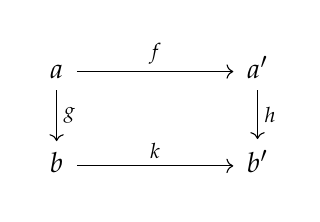
\begin{tikzpicture}
          \node {\begin{tikzcd}[column sep=20mm]
              a\ar[r,"f"]\ar[d,"g"] & a'\ar[d,"h"]\\
              b\ar[r,"k"] & b'
            \end{tikzcd}};
        \end{tikzpicture}
      \]
      \caption*{The square category.}
    \end{figure}

    Note that the elements $F:Sqr \to C$ are the collections of the arrows of the arrow category of $C$.
    
  \item We can use this construction to study the category $C^C$ of endofunctors of a particular category $C$. This case is particularly interesting while studying the endofunctors present in $Hask^{Hask}$ and later consider the Monad as a programming structure. 
  \end{itemize}
\end{example}

Note that this is not the only way in which to define the composition of natural transformations can be defined. In fact, we can define another functor category. In this case we compose two natural transformation as in:

\[
  \begin{tikzcd}[column sep=huge]
    B
    \arrow[bend left=40]{r}[name=F,label=above:$\scriptstyle F$]{}
    \arrow[bend right=40]{r}[name=G,label=below:$\scriptstyle G$]{} &
    C
    \arrow[bend left=40]{r}[name=F',label=above:$\scriptstyle F'$]{}
    \arrow[bend right=40]{r}[name=G',label=below:$\scriptstyle G'$]{}&
    D
    \arrow[shorten <=3pt,shorten >=3pt,Rightarrow,to path={(F) -- node[label=right:$\tau$] {} (G)}]{}
    \arrow[shorten <=3pt,shorten >=3pt,Rightarrow,to path={(F') -- node[label=right:$\sigma$] {} (G')}]{}
  \end{tikzcd}
\]

Lets formalize this composition:
\begin{definition}\label{horizontal-composition}
  Let $B,C,D$ be categories, $F,G: B \to C, F',G':C\to D$ be functors, and let $\tau: F \to G$, $\sigma:F'\to G'$, we define the horizontal composition $(\tau \circ \sigma): F\circ F' \to G\circ G'$ by: $$(\sigma \circ \tau) c = \sigma F c \circ G' \tau c$$  for all $c\in B$.
\end{definition}

In this case we can see that the composition of two natural transformation is indeed a natural transformation due to the commutativity of:

\[
  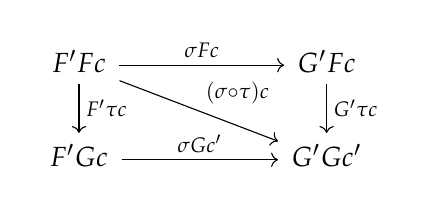
\begin{tikzpicture}
    \node {\begin{tikzcd}[column sep=20mm]
        F'Fc      \ar[r,"\sigma F c"]
        \ar[d,"F'\tau c"]
        \ar[dr,"(\sigma\circ \tau)c"]
        & G'Fc\ar[d,"G'\tau c"]\\
        F'Gc\ar[r,"\sigma Gc'"] & G'Gc'
      \end{tikzcd}};
  \end{tikzpicture}
\]


With this definition of composition we can consider another different category: the category of all functors of all (small) categories, that is, the category that has all the functors as object, and has the natural transformation with horizontal composition as arrows.\\

When we have to consider both compositions at the same time we denote the vertical composition with $\tau \cdot \sigma$ and horizontal composition with $\tau \circ \sigma$ , as in  \cite{mac2013categories}. Lastly we have to consider how this composition relate to each other. This is seen in the \emph{interchange law}:\\

\begin{proposition}
  Let $A,B,C$ be categories, let $F,G,H:A\to B$ and  $F',G',H':B\to C$ be functors and $\tau: F \to G,\sigma:G\to H,\tau': F' \to G'$ and $\sigma' : G'\to H'$ be natural transformations. Then:
  $$(\sigma' \circ \sigma)\cdot (\tau' \circ \tau) = (\sigma' \cdot \tau')\circ (\sigma\cdot \tau)  $$
\end{proposition}
\begin{proof}
  We have a structure like   

  \[
    \begin{tikzcd}[column sep=huge]
      A
      \arrow[bend left=60]{r}[name=F,label=above:$\scriptstyle F$]{}
      \arrow{r}[name=G,label=right above:$\scriptstyle G$]{}
      \arrow[bend right=60]{r}[name=H,label=below:$\scriptstyle H$]{}  &
      B
      \arrow[bend left=60]{r}[name=F',label=above:$\scriptstyle F'$]{}
      \arrow{r}[name=G',label=right above:$\scriptstyle G'$]{}
      \arrow[bend right=60]{r}[name=H',label=below:$\scriptstyle H'$]{}  &
      C
      \arrow[shorten <=3pt,shorten >=2pt,Rightarrow,to path={(F) -- node[label=left:$\tau$] {} (G)}]{}
      \arrow[shorten <=3pt,shorten >=2pt,Rightarrow,to path={(G) -- node[label=left:$\sigma$] {} (H)}]{}
      \arrow[shorten <=3pt,shorten >=2pt,Rightarrow,to path={(F') -- node[label=left:$\tau'$] {} (G')}]{}
      \arrow[shorten <=3pt,shorten >=2pt,Rightarrow,to path={(G') -- node[label=left:$\sigma'$] {} (H')}]{}
    \end{tikzcd}
  \]

  From the  naturality of $\tau'$ we have that for all $c\in A$:
  \begin{align*}
    ((\sigma'\cdot \tau')\circ (\sigma\cdot \tau))(c)
    & = H' ((\sigma\cdot \tau) c ) \circ (\sigma'\cdot \tau') (F c)  \\
    & = H' ( \sigma c \circ \tau c) \circ (\sigma' (Fc)\circ \tau' (F c) )  \\
    & = H' ( \sigma c) \circ H'(\tau c) \circ \sigma' (Fc)\circ \tau' (F c)   \\
    &  = H' ( \sigma c) \circ
      \sigma'Gc \circ G' \tau cH'(\tau c) \circ \sigma' (Fc)
      \circ \tau' (F c)   \\ 
    &  = (\sigma' \circ \sigma) (c) \circ  (\tau \circ \tau) (c)   \\
    &  = ((\sigma' \circ \sigma) \cdot  (\tau' \circ \tau)) (c). 
  \end{align*}
\end{proof}

To finally consider the relation between products, and the functor category we can see that given three small categories $A,B,C$ we have a bijection:

$$\hhom_{Cat}(A\times B, C) \cong \hhom_{Cat}(A, C^B).$$

This fact will be taken into account further in the text, as this will mean that the functor $\cdot \times B: Cat \to Cat$ has a right adjoint.
\subsubsection{Comma Category}

To define the comma category, we shall define the category $(b \downarrow S)$ of objects $S$-under $b$, sketch the dual notion, and generalize this two concepts with the comma category.\\

Given a functor $F:B\to C$ an object $b\in B$ is $F-$under another object $c\in C$ if there exists an arrow $f:c\to b \in C$. This can be represented as

$$
\begin{tikzcd}
  c
  \ar[d,"f"]\\
  Fb
\end{tikzcd}
$$

and thus the name of $F$-under.

\begin{definition}
  Let $B,C$ be  categories and $S:B\to C$ be a functor. For every $c\in Ob(C)$ we can define the category $(c \downarrow S)$ that has as objects all pairs $(b,f) \in Ob(B)\times Ar(C)$ where $f:c\to Sb$, and as arrows $h:(d,f) \to (d',f')$ the arrows $h:d\to d'\in Ar(B)$ such that $f' = Sh\circ f$.
\end{definition}

The property that each arrow should satisfy can be represented as:
\[
  \begin{tikzpicture}
    \node {\begin{tikzcd}
        & c\ar[ddl, "f"]\ar[ddr,"f'",swap] & \\
        &&\\
        Sd\ar[rr, "Sh", swap] & & Sd'
      \end{tikzcd}};
  \end{tikzpicture}
\]

\begin{example} Let $U:Grp \to Set$ be the forgetful functor, and let $X\in Ob(Set)$. We can consider $(X\downarrow U)$ where every object is a function of Sets $f: X\to Ug$ for a group $g$.  
\end{example}

One can easily now deduce the dual concept of the category $(b\uparrow S)$ represented by: \\
\begin{center}
  objects: $
  \begin{tikzcd}
    c
    \\
    Fb\ar[u,"f"]
  \end{tikzcd}
  $;$\qquad$ arrows: $\begin{tikzcd}
    & c & \\
    &&\\
    Sd\ar[rr, "Sh", swap]\ar[uur, "f"] & & Sd'\ar[uul,"f'",swap]
  \end{tikzcd}$.
\end{center}

Now suppose that we have three categories $B,C,D$ and two functors $S,T$ such that
\[
  \begin{tikzcd}
    B \ar[r, "S"] & C & D\ar[l, "T", swap]
  \end{tikzcd}
\]

We might want to consider the relations objects of $B$ and $D$, for that we have the comma category:


\begin{definition}
  Let $B,C,D$ be categories and to $S:B\to C,T: C\to D$. We define the coma category $(S\downarrow T)$ as the category that has as object the triples $(b,d,f)$ with $b\in Ob(B), d\in Ob(D), f:Sb\to Td\in Ar(C)$ and as arrows the pairs $(g,h):(b,d,f)\to (b',d',f')$ with $g:b\to b'\in Ar(B), h:d\to d'\in Ar(D)$ such that $Th \circ f = f' \circ Sg$. 
\end{definition}

We can represent the previous definition by:
\begin{center}
  objects: $
  \begin{tikzcd}
    Sb\ar[d,"f"]
    \\
    Td
  \end{tikzcd}
  $;$\qquad$ arrows: $\begin{tikzcd}
    Sb\ar[d,"f"]\ar[r,"Sg"] & Sb' \ar[d,"f'"]
    \\
    Td\ar[r,"Sh"] & Td'
  \end{tikzcd}$.
\end{center}


The name comma category comes from is alternative notation $(S\downarrow T) = (S,T)$. We prefer the $(S\downarrow T)$ as it is more clear, nonetheless it is clear that before modern text editor became popular, the original comma notation had a big plus.

\chapter{Universality, Adjoints and Closed Cartesian Categories}

In this chapter we are going to study universality and adjunctions. Despite a possible apparent difference in definitions, both have the same use: they are tools that, given an arrow selected in a category, allow us to uniquely select an arrow in another category, generally fulfilling some special property (if not, a functor would be enough). \\

We will start this section with the definition of universality, as well as the statement of Yoneda's lemma. Then, we present the concept of Adjunction. We will use these concepts to introduce new structures, in particular that of closed Cartesian category.


\section{Universality}
In this section we present the concept of universality. This concept is behind lots of mathematical properties. Intuitively, universality is an efficient way of expressing an one-to-one correspondence between arrows of different categories. This one-to-one relationship is usually expressed via ''given an arrow  $y$ it exists one and only one  arrow $x$ such that <insert your favorite universal property>''.\\

Lets do an introductory example. Probably the first contact that any mathematician has with universality is defining a function  $f:\mathbb R \to \mathbb R^2$. It is easy to see that defining such a function is equivalent to define two $g,h: \mathbb R \to \mathbb R$. Furthermore, those $g,h$ are unique for each $f$. This uniqueness is the flavor that attempts to capture the concept of universality. Other examples of unique existence are those that occur in quotient groups or in bases of vector spaces. \\

\begin{definition}\label{def:univ-arrow}
  Let $S: D \to C$ be a functor and $c \in Ob(C)$, an \emph{universal arrow}  from $c$ to $S$ is a pair $(d,u)$ with $d\in Ob(D), u:c \to Sd \in Ar(C)$, such that for every $(e,f)$ with $e\in Ob(D)$  and $f:c\to Sd$ there exists an unique $f':r,d\in Ar(D)$ such that $Sf'\circ u = f$.

\end{definition}
In a diagram:

\[
  \begin{tikzcd}
      c\arrow[r, "u"] \arrow[rd, "f", swap]      & Sd \arrow[d, "Sf'", dashed]& d\arrow[d,"f'"]\\
       &Se& e 
    \end{tikzcd}
  \]

  Note that an universal arrow $(d,u)$ induces the unique existence of an arrow in $D$, but with interesting properties via it relationship with $S$. Usually, to provide an universal arrow we will only define the functor $S:D\to C$ and the arrow $u:c\to Sd$, letting all other information be deduced from the context.\\



  The idea of universality is often regard via the notion of \emph{universal element}, in the special (and commonplace) case where $S:D\to Set$.

  \begin{definition}
    Let $S: D \to Set$, an \emph{universal element}  for $S$ is a pair $(r,e)$ with $r \in Ob(D), e \in   Sr$, such that for every $(d,x)$ with $d\in Ob(D), x\in Sd$, there is an unique arrow $f:r\to d\in D$ such that $(Sf)e = x$. 
  \end{definition}


    Note that having an universal element is a particular case of having an universal arrow. Considering $*$ the set with one point (as a category) an universal element is an universal arrow $*\to H$. This is clearly seen if we consider the diagram:
%      c\arrow[r, "u"] \arrow[rd, "f"]
    \[
  \begin{tikzcd}
     *\arrow[r, "u"] \arrow[rd, "f", swap] & Sr \arrow[d, "Sf", dashed]& r\arrow[d,"f"]\\
      &Sd& d 
    \end{tikzcd}
  \]

  where $*$ is helping us select the elements of $Sd$ and $Se$ to enforce the property.\\

  Conversely if $D$ has small homesets, we can consider an universal arrow to be a particular case of an universal element. With the same context as in \ref{def:univ-arrow} $(d,u: c\to Sd)$ is an universal arrow if, and only if, $(d, u\in  \hom_{D}(c, Sd))$ is an universal element.\\

  The point of having these such similar definition is to have different interfaces for the concept. While most result can be easily adapted, once we got to the examples is clear when to use each concept. 
  
  \begin{example}\ 
    \begin{itemize}
    \item Quotient Group: This property states that, for any two groups $N\lhd G$ with $\pi: G \to N$ the canonical projection, and any group homomorphism $f:G\to K$ such that $N\subset \ker f$ there exists an unique $\overline f: H \to K$ such that $\overline f  \circ \pi = f$.\\
      
      The question now is, how is this a universal property. This is an example of a universal element. Considering the functor $H: Grp\to Set$:
      $$HG' = \{f:G\to G'\in Ar(Grp) : F(N)=\{0\} \},$$
      
      Then, $(G/N, \pi)$ is an universal element for $H$. From this property alone the three isomorphism theorems can be deduced. Therefore, we only have to prove this result to have the full power of these theorems in any context (e.g. Rings, K-Algebra, or Topological spaces).
    \end{itemize}
  \end{example}

  Dualy, we can consider an \emph{universal arrow from $S$ to $c$} or simply universal arrow from $S$:
\begin{definition}\label{def:univ-arrow2}
  Let $S: D \to C$ be a functor and $c \in Ob(C)$, an \emph{universal arrow}  from $c$ to $S$ is a pair $(d,u)$ with $d\in Ob(D), u:c \to Sd \in Ar(C)$, such that for every $(e,f)$ with $e\in Ob(D)$  and $f:c\to Sd$ there exists an unique $f':r,d\in Ar(D)$ such that $u\circ Sf' = f$.

\end{definition}
In a diagram:

\[
  \begin{tikzcd}
      c       & Sd \arrow[swap, l, "f"]\arrow[d, "Sf'", dashed]& d\arrow[d,"f'"]\\
       &Se\arrow[lu, "u"]& e 
    \end{tikzcd}
  \]


  \begin{example}\ 
    \begin{itemize}
    \item In $Sets$ we have a particular construction: the product of sets for any two sets $a,b$ along with the projections $\pi_1 a \times b \to a$ and $\pi_2 a \times b \to b$. Then, we can define the functor $\Delta: Set \to Set\times Set$ such that $\Delta c = c\times c$ for every $c\in Ob(Set)$ and $\Delta (f:c\to b): c\times c\to b\times b$ is the elements-wise aplication of $f$.\\

Then, given any two sets $a,b\in Ob(Sets)$, $u=(\pi_1,\pi_2)$ is an universal arrow from $\Delta$ to $(a,b)$ as

\[
  \begin{tikzcd}
      (a,b)       & \Delta d=(d,d) \arrow[swap, l, "f"]\arrow[d, "\Delta f'", dashed]& d\arrow[d,"f'"]\\
       &\Delta e=(e,e)\arrow[lu, "u"]& e 
    \end{tikzcd}
  \]

\end{example}

    
  Lastly, we will provide a characterization of universality:
  \begin{proposition}\label{Yoneda-proposition}
      Let $S: D \to C$ be a functor and $u:c\to Sr\in Ar(C)$. Then $u$ is an universal arrow if and, only if, the function $\varphi:\hom_D(r,\cdot)\to \hom(c,S\cdot)$ such that $\varphi(d)(f)= Sf\circ u$ for all $f\in \hom_D(r,d)$ is a natural bijection. Conversely, every natural bijection is uniquely determined by an universal arrow $u:c\to Sr$. 
  \end{proposition}
  \begin{proof}
    Let $u$ be universal. Then for $\varphi$ to be a natural transformation the diagram 
    \[
      \begin{tikzcd}
        \hom_D(r,d)\arrow[swap]{d}{\hom_D(r,g)}\arrow{r}{\varphi(d)} & \hom_C(r,Sd)\arrow{d}{\hom_C(r,Sg)}\\
        \hom_D(r,d')\arrow{r}{\varphi(d')} & \hom_C(r,Sd')
      \end{tikzcd}
    \]

    should commute for all $g\in Ar(D)$. As this is a diagram in the category of sets, we can check the commutativity by checking it element wise. For any $f \in\hom_D(r,d)$:
    \[
      \begin{tikzcd}
        f\arrow[swap]{d}{\hom_D(r,g)}\arrow{r}{\varphi(d)} & Sf\circ u \arrow{d}{\hom_C(r,Sg)}\\
        g\circ f \arrow{r}{\varphi(d')} & S(g\circ f) \circ u = Sg\circ Sf \circ u
      \end{tikzcd}
    \]

    So the diagram commutes, and $\varphi$ is natural. The bijectivity follows from $u$ being universal.\\

    Lets consider now that $\varphi$ is a natural bijection. We will define $u := \varphi(r)(1_r)$ and check that $(r,u)$ is an universal arrow. As $\varphi$ is natural we have that:

    \[
      \begin{tikzcd}
        \hom_D(r,r)\arrow[swap]{d}{\hom_D(r,g)}\arrow{r}{\varphi(r)} & \hom_C(r,Sr)\arrow{d}{\hom_C(r,Sg)}\\
        \hom_D(r,d)\arrow{r}{\varphi(d)} & \hom_C(r,Sd)
      \end{tikzcd}
    \]

    Writing the diagram for the element $1_r\in\hom_D(r,r)$ and any $d\in Ob(D), g:r\to d\in \hom_D(r,d)$:

    \[
      \begin{tikzcd}
        1_r \arrow[swap]{d}{\hom_D(r,g)}\arrow{r}{\varphi(r)} & u \arrow{d}{\hom_C(r,Sg)}\\
        g\arrow{r}{\varphi(d)} & \varphi(d)(g)= Sg\circ u
      \end{tikzcd}
    \]

    and since $\varphi$ is a bijection, for every $f\in \hom_C(r,Sd)$ there is an unique function $f' = \varphi(d)^{-1}(f)$ such that $Sf'\circ u = f$, thus being $u$ universal.

\end{proof}
From this theorem there is a definition that arises:

\begin{definition}
  Let $D$ be a category with small home-sets and let $F:D\to C$ be a functor. A representation of a functor $K:D\to Set$ is a pair $(r,\varphi)$ with $r \in Ob(D)$ and $ \varphi$ a natural isomorphism  such that
  $$D(r,\cdot) \equiv_{\varphi} F.$$
  A functor is said to be \emph{representable} whenever it has a representation.
\end{definition}

Note that therefore a universal arrow induces a natural isomorphism $D(r,d)\equiv C(c,Sd)$ and this induces a representation of the functor $C(c,S\cdot): D\to Set$, being these three equivalent.

\subsection{Yoneda's lemma}
This subsection  deals with Yoneda's Lemma. Mac Lane\cite{mac2013categories} assures the lemma first appeared in his private communication with Yoneda in 1954. With time, this result has became one of the most relevant one in Category Spaces. We will start by providing some intuition to it, followed by it proof and some use cases.\\


 This results is due to japanese professor Nobuo Yoneda. We know about Yoneda's life thanks to the elegy that was written by Yoshiki Kinoshita\cite{YonedaLife}. Yoneda was born in Japan in 1930, and received his doctorate in mathematics from Tokyo University in 1952. He was a reviewer for international mathematical journals. In addition to his contributions to the field of mathematics, he also devoted his research to computer science.\\


The idea behind the Yoneda lemma can be arid at first, if one does not have a prior understanding of what the purpose and usefulness of this lemma is. In order to ilustrate this idea we will introduce a (simplified) definition of Moduli Spaces, so that we have a geometric understanding of Yoneda's Lemma.\\

The idea behind (some) Moduli spaces is to classify algebraic curves up to isomorphisms. In addition, Moduli spaces allow us to control complex mathematical objects (such as a quotient space of unknown objects) by simpler objects or objects with better properties (such as a concrete variety). A canonical example of this type of classification is:  
\begin{align*}
  \{\text{Vector spaces of finite dimension}\}/\text{isomorphism } &\cong \N\\
  [V] &\to dim V.
\end{align*}
Where a complex object can be classified by another object of which we know more properties. We can start by defining:  
$$\mathcal{M} = \{\text{smooth complex non singular curves} \}/\text{isomorphism}$$

Further on when we talk about curves we will refer to smooth complex non singular curves. Note that if two curves are isomorphic then they have the same genus. Therefore the function 
\begin{align*}
      \gamma: \mathcal{M} &\mapsto \N\\
      \displaystyle  [V]&\mapsto \text{genus of V} 
\end{align*}

is well defined and we can define $\mathcal{M}_g = \gamma^{-1}(g)$. An interesting classification of $\mathcal{M}_g$ is given when we consider that for every $g$ there exists a closed, connected, non-singular variety $U_g$ and a family $\{C_t : t \in U_g}$ such that a curve of genus $g$ will be a fibration of $C_t$.  Moreover there is a variety $M_g$ and a superjjective morphism $\varphi: U_g \to M_g$ such that $\varphi(t_1)=\varphi(t_2)$ if $C_{t_1} \equiv C_{t_2}$. Therefore we are classifying the equivalence classes of $\mathcal{M}_g$ by points of the variety $M_g$ (thus generating a Moduli problem).\\

Similarly to this two example, with the Yoneda lemma we will have a functor $F:D\to Set$ and one representation of this functor. We will classify the natural transformation of these functors by the set in the image of $F$! Interestingly enough, there will be applications where the complex object is not the space of naturals transformations, but the images of $F$ (see \ref{Cayleys} for an example). Lets proceed to enunciate and proof the result.

\begin{theorem}\cite[Section 3.2]{mac2013categories}
  Let $D$ be a category with small home-sets, $F:D\to Set$ be a functor, and $r\in Ob(D)$. Then there is a bijection
  \begin{align*}
    \tau:Nat(\hom_D(r,\cdot), F\cdot) &\equiv Fr\\
    \tau(\alpha:\hom_D(r,\cdot)\to F\cdot)& = \alpha(r)(1_r)
  \end{align*}
  Where $\tau$ is natural in $K$(as an object of $Set^{D}$) and in $r$.
\end{theorem}
\begin{proof}
  As $\alpha$ is a natural transformation we have that, for every $g:r\to d\in Ar(D)$: 
    \[
      \begin{tikzcd}
        \hom_D(r,r)\arrow[swap]{d}{\hom_D(r,g)}\arrow{r}{\alpha(r)} & Kr\arrow{d}{Kg}\\
        \hom_D(r,d)\arrow{r}{\alpha(d)} & Kd
      \end{tikzcd}
    \]
Writing $\alpha(r)(1_r) = u$ we have that:
    \[
      \begin{tikzcd}
        1_r\arrow[swap]{d}{\hom_D(r,g)}\arrow{r}{\alpha(r)} & u\arrow{d}{Kg}\\
        g\arrow{r}{\alpha(d)} & \alpha(d)(g)=Kg(u)
      \end{tikzcd}
    \]

    Therefore every natural transformation is uniquely identified by the value of $u$, therefore $\tau$ is injective. Moreover, for every $u$ in $Kr$, we can define a natural transformation following the previous diagram, therefore, $\tau$ is bijective.\\

To see that $\tau$ we is natural we have to consider for which functor it is natural. Consider the functor \emph{Evaluation} $E: Set^D\times D$ that maps each $(F,c)\to Fc$, and the functor $N:Set^D\times D\to Nat(\hom_D(r,\cdot),K)$ the set of natural transformations. Finally, $\tau:N\to E$ is a natural transformation.
\end{proof}

The first functor that we will want to apply this result is to the $\hom_{\cdot}$ functor. But this functor is a bifunctor, so to get the full result of this lemma applied to the full bifunctor we may restate this lemma to contravariant functors.

\begin{corollary}
  Let $D$ be a category with small home-sets, $F:D\to Set$ be a contravariant functor, and $r\in Ob(D)$. Then there is a bijection
  \begin{align*}
    \tau:Nat(\hom_D(\cdot,r), F\cdot) &\equiv Fr\\
    \tau(\alpha:\hom_D(\cdot,r)\to F\cdot)& = \alpha(r)(1_r)
  \end{align*}
  
  Where $\tau$ is natural in $K$(as an object of $Set^{D}$) and in $r$.
\end{corollary}
\begin{proof}
We seek to use the Yoneda lemma in the functor $F':D^{op}\to Set$ induced by $F$. Then we have that: 
  \begin{align*}
    \tau:Nat(\hom_{D^{op}}(r,\cdot), F'\cdot) &\equiv F'r\\
    \tau(\alpha:\hom_{D^{op}}(r,\cdot)\to F'\cdot)& = \alpha(r)(1_r)
  \end{align*}

  Taking into account that $F_{|Ob(D)}=F'_{|Ob(D^{op})}$, and that 
  $\hom_{D^{op}}(r,\cdot) = \hom_D(\cdot,r)$ we have the result.
\end{proof}

As we have seen, the Yoneda lemma is a direct generalization of the moduli problem. In the same vein, Yoneda's lemma is the generalisation of other problems/theorems in mathematics, most notably Cayley's lemma. It states:
\begin{proposition} \label{Cayleys}
Any group is isomorphic to a subgroup of a symmetric group.
\end{proposition}

To understand this, take a groups $G$ seen as a single-object category, and name that object $e$. Then, the functor $\hom_G(e, \cdot): G \to Set$ can be seen as a group action \ref{group-action}. Then the Yoneda lemma states that:

$$Nat(\hom_G(e,\cdot), Hom_G(e,\cdot)) \equiv_\varphi Hom_G(e,e).$$

Translating this result to group theory:
\begin{itemize}
\item Remember that $Hom_G(e,e)$ is the group $G$.
\item Every natural transformation is a equivariant map between G-sets.
\item This equivariant maps, forms an endormophism group under composition, being a subgroup of the group of permutations.
\item This natural isomorphism $\varphi$ define a group isomorphism.
\end{itemize}

So we have the isomorphism of groups that is stated in Cayley's Theorem.\\



We continue our exploration of Yoneda lemma by defining the \emph{Yoneda Embedding}. For that we define the contravariant functor $h_a = \hom_C(\cdot, a)$. Then the contravariant Yoneda lemma tell us that:
$$Nat(h_a,h_b) \equiv_{\tau_a} \hom(a,b).$$

We then can define a fully faithfull embedding $\upsilon: C \to Set^{C^{op}}$ such that 
\begin{align*}
  \upsilon a  &= \hom_C(A, \cdot)\qquad \forall a \in Ob(C), \\
  \upsilon f &= \tau_a^{-1} (f)\qquad\qquad \forall f:b\to a\in Ar(C).
\end{align*}

This functor allows us to view the category $C$ as a subcategory of the category of contravariant functors from $C$ to $Set$, which will be useful for determining "heritable" properties in $C$.
\subsection{Properties expressed in terms of universality}

  After the examples given, we define a few constructions that are commonplace in Maths. We will outline the notions of limit, pullback and product, and the dual notions of colimit, pushout and coproduct.\\

  The notions of product and pullback can be seen as particular cases of the notion of limit. To define limit we will introduce the concept of co-cone and the diagonal functor. \\

  \begin{definition}
    Let $C,J$ be categories. We can define the functor $\Delta_J: C \to C^J$ that maps $c$ to the functor from $J$ to $C$ that is constantly $c$, and maps every arrow to the identity $1_c$. 
  \end{definition}

  Whenever possible we will write only $\Delta$, and let the information of the category be deduced from context. $J$ is usually small and often finite. We can now consider a natural transformation $\tau: F \to \Delta c$. This can be represented as in the following diagram:
    \[
      \begin{tikzcd}
        Fx_j\arrow[swap]{dr}{\tau x_j}\arrow{rr}{F g} &
        & Fx_k\arrow{dl}{\tau x_k}\\
        & c&
      \end{tikzcd}
    \]

    commutes for every $g:x_j\to x_k\in Ar(j)$, for that reason, such natural transformation is usually called a co-cone. The dual notion is called cone and  is represented as:
    \[
      \begin{tikzcd}
        Fx_j\arrow{rr}{F g}&
        & Fx_k\\
        & c\arrow{ur}[swap]{\tau x_k}\arrow{ul}{\tau x_j} &
      \end{tikzcd}
    \]


    We can now define the concepts of limit and colimit. We introduce first the concept of colimit. This definition is that of an universal arrow, only in a category of functors. Following this definition, we will define the limit as its dual concept.
  \begin{definition}
 A colimit is an object $r\in Ob(C)$ together with an universal arrow $u:F\to \Delta r \in Ar(C^J)$. The colimit is denoted by $$\lim_{\leftarrow} F = r = \colim F.$$
  \end{definition}

  The notation $\lim_{\leftarrow}$ is intuitive: in the colimit we have arrows to $F$. To represent this as a diagram, we have a co-cone $u\to \colim F$ such that for every other co-cone $\tau \to s$, it exist an unique $f$ such that the following commutes for every $x_j,x_k\in Ob(C)$:

\[
\begin{tikzcd}
{} & l& & \\
& \colim F   \arrow[dashed]{u}[description]{f} \\
x_j \arrow{ur}{u x_j} \arrow[bend left]{uur}{\tau x_j}\arrow[swap]{rr}{Fg} & & 
x_k \arrow[swap]{dr}{u x_k}\arrow[bend right,swap]{uul}{\tau x_k}\\
\end{tikzcd}
\]

  
Now, thanks to the duality of categories, we can define what a limit is in a very synthetic way:

\begin{definition}
  A limit is the dual concept of a colimit. It is denoted as
  $$\lim_{\rightarrow} F = r = \lim F.$$
\end{definition}

A limit is represented by the following diagram:
\[
\begin{tikzcd}
{} & l
\arrow[bend right,swap]{ddl}{\tau x_j}
\arrow[bend left]{ddr}{\tau x_j} \arrow[dashed]{d}[description]{f}& & \\
& \lim F \arrow{dr}{u x_k} \arrow{dl}[swap]{u x_j} \\
x_j \arrow[swap]{rr}{Fg} & & 
x_k \\
\end{tikzcd}
\]

Analogously as in the colimit notation, in the limit we have arrows from $F$, and thus the notation $\lim_{\rightarrow}$. Let focus for a while now in the notion of limit, in particular of two of its specials cases: the product and the pullback. From these cases we are going to provide most examples. \\

We have already talked about the product of categories, and in example \ref{example product} we denote that in these type of construction there is some sort of universality involved. The product is a limit where $J$ is the 2-element discrete category, that is, where every functor $F:J\to C$ is merely choosing to object of $C$. 

\begin{definition}\label{prod-univ}
  Let $C$ be a category, $J=\{0,1\}$ be the discrete category with two elements. The product $c_1\times c_2$ of two elements $c_0,c_1\in Ob(C)$ is the limit of the functor $F:J\to C$ such that $F0 = c_0, F1= c_1$.
\end{definition}

This construction means that providing an arrow to $c_0,c_1$ determines an unique arrow to $c_0\times c_1$. In this case, the arrows $u0, u1$ are usually called \emph{projections} and denoted by $\pi_0, \pi_1$. The notation is due to the product being a generalization of the cartesian product in the category $Set$. It is also sometimes note with $c_0 \Pi c_1$ with $\Pi$ being stardard for the sequence product. Some examples of product object in categories are:
\begin{example}\ 
\begin{itemize}
\item Product of Banach spaces:
\item Product of something in haskell.
\end{itemize}
\end{example}

Analogously, we can define the coproduct, on which instead of defining an arrow to $c_0, c_1$, we define an object \emph{from} $c_0,c_1$. 
\begin{definition}
  The coproduct is the dual definition of the product. It is denoted by $c_0 \sqcup c_1$.
\end{definition}
 In this notation $\sqcup$ denotes an inverted $\Pi$, with the meaning of being the dual notion of the product.
\begin{example}\ 
  \begin{itemize}
  \item Tensor Product of R-Modules, include cite to Rotman-Theorem 1.5.
  \item Union of enumerate types.
  \end{itemize}
\end{example}



% From my personal experience I have to say that I have seen more difficulties learning this notion rather than learning the utterly similar notion of product, probably because we are more used to think in terms of arrays rather than in terms of universality for the product. I think that thinking in terms of universality should be the way in to these concept.


After learning about the product and the coproduct, we will focus now in the notion of pullback and its dual, the pushout. We will first define the category

\[
  P = \begin{tikzcd}
    x\arrow{r}{f} & z & y\arrow[swap]{l}{g}
\end{tikzcd}
\]

Then we can define the pullback:

\begin{definition}
  Let $C$ be a category and $F:P\to C$ be a functor. Then the pullback of $Fx$ and $F_y$ denoted as $Fx\times_{Fz}Fy$ is the limit of the functor $F$.
\end{definition}

We can represent this structure in the following diagram. For any object $q$ and arrows $f':q\to Fx,g':q\to Fy$ we have:

\[
\begin{tikzcd}
q
\arrow[bend left]{drr}{g'}
\arrow[bend right,swap]{ddr}{f'}
\arrow[dashed]{dr}[description]{u} & & \\
& Fx\times_{Fz}Fy \arrow{r}{p_2} \arrow{d}[swap]{p_1}
& Fy \arrow{d}{Fg} \\
& Fx \arrow[swap]{r}{Ff}
& Fz
\end{tikzcd}
\]

Analogously, we can define:

\[
  CoP = \begin{tikzcd}
    x & z\arrow{l}{f}\arrow[swap]{r}{g} & y
\end{tikzcd}
\]

and define:
\begin{definition}
  Let $C$ be a category and $F:CoP\to C$ be a functor. Then the pushout of $Fx$ and $F_y$ denoted as $Fx\sqcup_{Fz}Fy$ is the colimit of the functor $F$.
\end{definition}

\begin{example}
  \begin{itemize}
  \item Fiber bundles (pullback)
  \item Suppose that X, Y, and Z as above are sets, and that f : Z → X and g : Z → Y are set functions. The pushout of f and g is the disjoint union of X and Y, where elements sharing a common preimage (in Z)
   \item Seifert-Van-Kampen (Si tienes valor).
  \end{itemize}
\end{example}

Note the  similarity of the pullback/pushout and the one of product/coproduct notation-wise. To understand these we have to consider the similarities of both construction. We are going to focus on the similarities of product and pullback, letting the coproduct/pushouts as duals.\\

In both case, the universal property consists of having an arrow to a generated object only if we have an arrow to each of its generators. In this line of reasoning, we can consider that the product is a pullback where we forget about the object $z$ and its arrows. One easy way to generate that case is to consider the construction when $Fz$ is a terminal object. In that case we have that the existence of $Ff$ and $Fg$ is a tautology, and we can consider 

\[
\begin{tikzcd}
& q
\arrow[bend left]{dr}{q_2}
\arrow[bend right,swap]{dl}{q_1}
\arrow[dashed]{d}[description]{u} & & \\
 Fx  & Fx\times_{Fz}Fy \arrow{r}{\pi_1} \arrow{l}[swap]{\pi_0}& Fy \\
\end{tikzcd}
\]

% having a product structure.  One can proceed to consider an analogous consideration with pushout and coproduct.\\



% One last property that can be expressed in terms of universality, and in particular in terms of limit/colimit is the \emph{power/copower}. The first example of power that we have considered yet of such construction is, given $C$ a small categories an $J$ a discrete category, the category $C^J$ is the power of $C$ up to $J$. The notation is due to the standard tuple notation:  considering a set of  tuples in $\R^n$, is in fact the same as considering the functions from  $n= {0,...,n-1}$ to $\R$.\\

% There are two intuitive notion behind this definition:
% \begin{itemize}
% \item The one more close to the formalism: to consider as a infinite product of the same element.
% \item To consider this 
% \end{itemize}



\section{Adjoints}

The adjoints is a fundamental property on Category theory. It relates two functors $F:C\to D, G:D\to C$. The importance of adjoints however, comes from it ubiquity among mathematics, often relate with the ubiquity of universality. This notion was first presented by Daniel M. Kan in \cite{kan1958adjoint}. For this section we follow \cite{mac2013categories}.\\

We  will start by providing some intuitive notions, before a formal definition. Take the Forgetful Functor $U:Grp\to Set$, and the Free Group Functor $\mathcal{F}:Set\to Grp$. We can see that it is not difficult to consider that we can compose $F$ and $G$ to make endofunctors. These endofunctors are far from being identities, nonetheless we have still a great relation between them: for every set $X$ and group $G$, there is a function $X \to UG$ for each morphism $FX\to U$. Conversely, any function from $X$ to $UG$ induces a morphism. \\

Any avid reader will detect by this point the taste of universality. But there is a bit more, we have a bijective relation on every image home-set of both $F$ and $G$. This is the underlying property of adjointness - to relate home-sets. Lets formalize this idea:
\begin{definition}
  Let $C,D$ be categories. And adjunction is a triple $(F,G,\varphi):D\to C$ where $F,G$ are functors:
  \[
    \begin{tikzcd}
      D\arrow[r, shift left=.5ex, "G"{name=F}] &
      C\arrow[l, shift left=1ex, "F"{name=G}] \\
    \end{tikzcd}
  \]
  while $\varphi$ is a transformation that maps each $(c,d) \in Ob(C\times D)$ with a bijection:
  \[
    \varphi_{c,d}:\hom_C(Fd, c)\equiv\hom_D(d, Gc).
  \]
  which is natural in $c$ and $d$.
\end{definition}

We have a bit to unpack in this definition. We will start to understand in what sense $\varphi$ is natural. Remembering about $N$ functor in Yoneda's Lemma, we can see that it is natural bijection from $\varphi:Hom_C(F\cdot, \cdot)\to \hom_D(\cdot, G\cdot)$ in each variable. That is,  for every $f:d\to d'\in C,k:c\to c' \in D$ the diagrams

\[
\begin{tikzcd}
 \hom_C(Fd,c) \arrow{d}{\hom_C(Fd,\cdot)(g)}\arrow{r}{\varphi_{c,d}}
 &\hom_D(d,Gc)\arrow{d}{\hom_D(d,G\cdot)(g)}&
   \hom_C(Fd,c) \arrow{d}{\hom_C(F\cdot,c)(f)}\arrow{r}{\varphi_{c,d}}
    &\hom_D(d,Gc)\arrow{d}{\hom_D(\cdot,Gc)(f)}\\
 \hom_C(Fd,c') \arrow{r}{\varphi_{c',d}}  &\hom_D(d,Gc')&
    \hom_C(Fd,c') \arrow{r}{\varphi_{c,d'}}  &\hom_D(d,Gc')
  \end{tikzcd}
\]

comutes. \\

We can follow by considering the important notation decision: how to call the adjoints. This is a quite ambiguous notation, but we will stick with the notation of $F$ being the \emph{left adjoint} and $G$ being the \emph{right adjoint}. When a functor \emph{is} a left (resp. right) adjoint it \emph{has} a right (resp. left) adjoint. This notation comes from where is the functor placed in the home-set, when making the bijection.\\

We have already suggested the relationship between universality and adjointness. We can summary that relation in the following property:
\begin{proposition}
  An adjunction $(F,G,\varphi): D\to C $ determines:
  \begin{itemize}
  \item a natural transformation $\eta: I_D \to GF$ such that $\eta(x):x\to G$ is universal for every $x\in Ob(D)$. Conversely, we can define:
    $$\varphi(f:Fd\to c) = Gf\circ \eta(d): d\to G c.$$
  \item a natural transformation $\epsilon: FG\to I_C$ such that $\varepsilon(x):Fx\to a$ is universal for every $x\in Ob(C)$. Conversely, we can define:
    $$\varphi(g:d\to Gc) = \eta(c)\circ Fg: Fd\to c.$$
  \end{itemize}
\end{proposition}
\begin{proof}
  \begin{itemize}
  \item Let $a=Fd$, then we have that
    $$\hom_C(a, c)\equiv\hom_D(d, Gc).$$

    and by proposition \ref{Yoneda-proposition} we have an universal arrow $\eta (d):d\to Ga=GFd$ is provided. The function $d\to \eta(d)$ is natural $I_D\to GF$ as:
    \[
  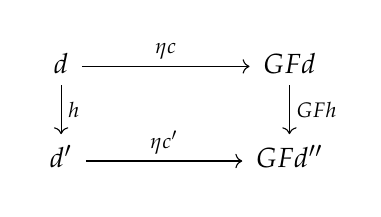
\begin{tikzpicture}
  \node {\begin{tikzcd}[column sep=20mm]
      d\ar[r,"\eta c"]\ar[d,"h"] & GFd\ar[d,"GFh"]\\
      d'\ar[r,"\eta c'"] & GFd''
  \end{tikzcd}};
\end{tikzpicture}
\]
commutes. 
  \item Analogous.
  \end{itemize} 
\end{proof}


From this proposition we can see that we may be able to define an adjoint based only on the universal arrows provided. We can summary a few equivalent definition of adjoint:
\begin{proposition}
  Each adjoint $(F,G,\varphi,\eta,\varepsilon):D\to C$ is completely determined by the items in any one of the following list:
  \begin{enumerate}
  \item $F,G$ and a natural transformation $\eta:1_D\to GF$ such that $\eta(d)$ is universal for every $d\in \Ob(D)$.
  \item $F,G$ and a natural transformation $\varepsilon:FG\to 1_C$ such that $\varepsilon(c)$ is universal for every $c\in \Ob(C)$.
  \item $G$ and for each $d\in Ob(D)$:
    \begin{itemize}
    \item an object $F_0(d)\in Ob(C)$.
    \item an universal arrow $\nu(x):d \to GF_0 d$.
    \end{itemize}
    Then $F$ has $F_0$ as object function and $F(h:d\to d') = \eta(x')\circ h$.
  \item $F$ and for each $c\in Ob(C)$:
    \begin{itemize}
    \item an object $G_0(c)\in Ob(D)$.
    \item an universal arrow $\varepsilon(c):c \to GF_0 c$.
    \end{itemize}
  \item  $F,G$ and two natural tranformation $\eta: I_D\to GF$, $\varepsilon: FG\to I_C$ such that both composites are identities.
  \end{enumerate}
\end{proposition}
\begin{proof}
  \begin{enumerate}
    
  \item We need to define the natural bijection $\varphi: C(Fd,c)\to D(d,Gc)$. Defining  $\varphi(g) = Gg\circ \eta(c)$ for each $g:Fd \to c$. Is is well define as $Gg\circ \eta(c): d\to Gc$ and it is a bijection  due to $\eta(x)$ universality.\\

    It is natural in $d$ because $\eta$ is natural and is natural in $c$ beacuse $G$ s a functor.
  \item Dual of the previous.
  \item We will proof that there is only one functor with $F_0$ as object function such that $\eta (x): I_D\to GF$ is natural. The naturality and universality told us that each $h:d\to d'\in Ob(D)$ induces two arrows:
\[
\begin{tikzcd}
  F_0 d\arrow[dashed]{d} & d\arrow{d}{h}\arrow{r}{\eta (d)}&GF_0d\arrow[dashed]{d}\\
  F_0 d'& d'\arrow{r}{\eta (d')} & GF_0d'
\end{tikzcd}
\]
    So the only way to define $Fh= \eta (x) \circ h$. We conclude applying 1.
  \item Dual of the previous.
  \end{enumerate}
\end{proof}
To further ilustrate this concept we present some examples:
\begin{example}
  \begin{itemize}
  \item Free group and forgetful functor
  \item \v{C}ech compactification.
  \end{itemize}
\end{example}

{\color{red} TODO? Lastly, we are going to study the  and prove a theorem that allow us to include parameters in adjoints.}



\subsection{Equivalente of Categories}
We can define an isomorphism of categories the same way that we define isomorphisms in any other category: an isomorphism is an arrow (Functor) with a two sided inverse. This definition, while standard, is quite restrictive. We are going to need some more lax concept of equivalence of categories, in the sense that while not being exactly the same, they are mostly the same. Formally:

\begin{definition}
A functor $F:C\to D$ is an equivalence of categories if there exists a functor $G:D\to C$  and two natural isomorphisms $\varphi: I_C \to GF$ and $\zeta: I_D\to FG$
\end{definition}


For the canonical example we may introduce a really organic concept: the \emph{skeleton} of a category. Quite often in mathematics we do not consider all objects of certain type, but rather objects up to isomorphism. The skeleton category of a category $C$ is another category where we consider the objects up to isomorphism. Formally:
  \begin{definition}
    Let $C$ be a category. The skeleton of $C$, namely $ske(C)$, is a subcategory  such that every object in $C$ is isomorphic to an object in $ske(C)$.
  \end{definition}

  The definition of equivalence of categories previously outline will allow us, for example, to consider $C\sim ske(C)$, while not being isomorphic. Continuing our discussion, it is not difficult to draw similarities between equivalences and adjoints. That motivates the further definition:
  \begin{definition}
    Let $(F,G,\varphi,\eta,\varepsilon)$ be an adjoint. It is called an \emph{adjoint equivalence} whenever $\eta$ and $\varepsilon$ are natural equivalences.
  \end{definition}
  It is clear that every adjoint equivalence induces two equivalences in $F$ and $G$. We state this idea in the following proposition:
  \begin{proposition}\cite[Theorem 1, 4.4]{mac2013categories}
    Let $F:C\to D$ be a functor. Then the following properties are equivalent:
    \begin{itemize}
    \item[i)] $F$ is an equivalence of categories.
    \item[ii)] $F$ is part of an adjoint equivalence. 
    \item[iii)] $F$ is full and faithfull, and each object $c\in C$ is isomorphic to $Sa$ for some object $a\in A$. 
    \end{itemize}  
  \end{proposition}
  \begin{proof}\
    \

    
    \begin{itemize}
    \item[$ii)\implies i)$] Given an equivalent adjoint $(F,G,\varphi,\eta,\varepsilon)$, then $F$ is an equivalence with $G,\eta,\varepsilon$. 
    \item[$i)\implies iii)$] $\varphi: GF\equiv I_C$ implies that for every $c\in Ob(C)$ we can consider $c\equiv GFc$. Then considering the natural isomorphism $\zeta: FG\equiv I_D$ states for every $f:a\to a'\in D$
\[
\begin{tikzcd}
  FGa \arrow{d}{FG f}& a\arrow{d}{f}\arrow{l}{\zeta^{-1} a}\\
  FGa' \arrow{r}{\zeta a'}& a'
\end{tikzcd}
\]

 there is one $FG f$ for each $f$ and we get that $G$ is faithful. Analagously we can see that $F$ is also faithful. To see that $G$ is full we can 
    \item[$iii)\implies ii)$] We can see that 
    \end{itemize}
  \end{proof}


  In the next few subsection, we are going to introduce categories, with some additional structures onto them. This type of considerations, are commonplace in category theory, and will provide useful considerations.

  \subsection{Monad}
  


  \subsection{Closed Cartesian Categories}

  The notion of product seen in \ref{prod-univ} is a notion that seek to catch the essence of what the Cartesian product is in the category of Set. In this category it happens that for any two objects, one can consider the product without any hesitance about it existence. A \emph{cartesian category} will be a category that, in some sense, maintain this property (of being closed under catersian product). Formally: 
  \begin{definition}
    A cartesian cartesian is a category for which every finite product exists.
  \end{definition}

Nonetheless, further on the text we will need categories with some even nicer properties. These categories are called \emph{closed catersian categories}. We will define them formally first, and after unpack the information that the definition contains:
  
  \begin{definition}
    A $C$ is closed cartesian if each of the following functors:
\begin{center}
  \begin{tabular}{p{0.3\linewidth}p{0.3\linewidth}p{0.3\linewidth}}
    $\qquad F_1:C\to 1$&$ F_2=\Delta: C \to C\times C $&$ F_{3}^b:C \to C$\\
    $\qquad \qquad c\to e$&$ \qquad \qquad c \to  (c,c)$&$ \qquad c \to c\times b$\\
  \end{tabular}
\end{center}
has a \emph{specified} right adjoint, denoted by:
\begin{center}
  \begin{tabular}{p{0.3\linewidth}p{0.3\linewidth}p{0.3\linewidth}}
    $\qquad G_1:1\to C$&$ G_2:  C\times C\to C $&$ G_{3}^b:C \to C$\\
    $\qquad \qquad e\to t$&$ \  \qquad (c,b)\to c \times b$&$ \qquad c \to c^b$\\
  \end{tabular}
\end{center}

These adjoints provide us with a lot of information:
\begin{itemize}
\item From $F_1$ being an adjoint we get that $t$ is terminal as for every $c\in Ob(C)$:
  $$\{id_e\} \equiv \hom_1(F_1(c), e) \equiv \hom_C(c,Ge=t)   $$
\item From $F_2$ we get that every pair $c,b$ has a product at is states the universal property of product:
  $$\hom_{C\times C}(F_2(c), (c',b'))\equiv \hom_{C\times C}((c,c), (c',b')) \equiv \hom_C(c,c'\times b')$$
  that is, for every object in $c\in C$, to provide a morphism to $c\to c'\times b'$ is the same that providing to morphisms $c\to c',c\to b'$.
\item First of all, as every product exists, and it specified by $F_2$, we can define $F_3^b$ for every $b$. Then, it adjointness states that:
  $$\hom_C(c\times b, d) \equiv \hom_C(c,d^b)   $$

  This object $d^b$ is called the exponential object or map object. The intuitive notion is that this object represent in some way the arrows from $b$ to $c$, being a generalization of the function set of two small sets. The best way to understand this adjoint is by the natural transformation $\varepsilon^b(c^b\times b) = c$. In this context, this is called \emph{evaluation arrow}. In the context of $Set$ this amount to the classic evaluation of a function.\\

actually it is a technical condition that this adjoint is natural in $b$ (cita maclane).
\end{itemize}

Lets provide some examples:

\begin{example}
  \begin{itemize}
  \item $Set$
  \item The category of compactly generated Hausdorff spaces.
  \item We will prove later that lambda calculus is, in some sense, a closed cartesian category.
  \end{itemize}
\end{example}



\part{Type Theory}
\label{Part2}


\part{Lambda Calculus}
\label{Part2}

\chapter{Lambda Calculus}

In this we will define the lambda calculus as a formal language of computation, and on this define the concept of typing, ubiquitous in programming languages. We will carry out this project raising as many bridges between category theory and the lambda calculus as possible.\\

The main references for this chapter are \cite{selinger2008lecture} for the general approach and concepts relatives to untyped calculus, \cite{lambek1988introduction} for more specifics details and the category theory approach to the calculus. We refer to \cite{cardone2006history} to further understand the historical motivation for the development of the theory.  \\


One of the important advances in 19th century mathematics is the development of the concept of function. However, what makes two functions the same? The most widespread view is the \emph{extensional} approach. In this, we consider two functions to be the same if for the same input they have the same output. In this case, the functions exist by themselves, and each $f$ as a pairing of an X domain to an Y codomain. These functions can  be considered as sets $f\subset X \times Y$.\\

Despite that, specially those involved in computing the functions, can consider this notion of equality misleading. For example, consider a prime $p$ big enough, and let $f$ and $g$ be two endomorphisms of  $\mathbb{Z}/p\mathbb{Z}$. One could argue that the endomorphism of  $f(x)\to x^2$ is different to $g(x) \to \log_a a^{x+2}$. Despite having the same output for the same input, one is clearly different in complexity. It even involve the resolution of a discrete logarithm, that is highly non trivial. \\

This view, in which not only is the result of the function important but how is that result obtained, is called the \emph{intensional} approach. This approach, gain traction in early 1930 as Church\cite{church1932set}, Gödel\cite{adams2011early} or Turing\cite{turing1938computable} start formalizing what is to be computable. This approach is now as ubiquitous modern computer program care not only on the correctness of a program, but on its time and space complexity (to the point on which correctness is often partially dropped to easy time complexity, for example \cite{hofmeister2002probabilistic}). \\

In lambda calculus we consider function as formulas, and thus, we consider an intensional approach. This intensional approach was also backed by the constructivist, to whom we will later on relate with the study of the Curry-Howard isomorphism  \cite{howard1980formulae}.\\


\section{Untyped Lambda Calculus }
We will start defining the most simple version of lambda calculus: untyped lambda calculus. Let's define some concepts:


\begin{enumerate}
\item An alphabet $A$ is an arbitrary, maybe finite, non-empty set.
\item A symbol $a$ in an element of the alphabet.
\item A word/formula is a finite sequence of symbols.
\item The collection of all possible words over an alphabet $A$ is denoted by $A^*$.
\item A language $L$ over $A$  is a subset of $A^*.$
\end{enumerate}

There are a lot of languages. For example, Spanish is a language, with a well-known alphabet $L$, with a proper subset of words over $L^*$.In the same fashion, we define lambda calculus as a formal language, defining its syntax, that is, what words are valid. After that, we will provide the semantics of the language, that is, we will provide meaning to the words.\\


\subsubsection{Syntax of untyped $\lambda$-calculus}
We start with the basic building blocks, which collectively form what is
called the alphabet:

\begin{itemize}
\item We denoted $x, y, z,...$ for variables. As more variables are necessary sub-indexes will be used, up to countable infinite variables.
\item We consider a abstractor connector $\lambda$.
\end{itemize}
Now, we are ready to formally define the untyped $\lambda$-calculus:

\begin{definition}[Syntax of Untyped $\lambda$-calculus (section 2.1 \cite{selinger2008lecture})]\label{def:untyped-lambda-calc}
  A $\lambda$-calculus formula (sometimes called term) is defined inductively:
  \begin{itemize}
  \item Every variable $x,y,z...$ is a valid formula.
  \item If $A,B$ is a formula, then $AB$ is a valid formula.
  \item If $A$ is a formula and $x$ is a variable, then $\lambda x.M$ is a valid formula.
  \end{itemize}
  The set of all variables is denoted by $\mathcal{V}$ and the set of all $\lambda$-formulas is denoted by $\Lambda$.\\
\end{definition}


Dealing with formal languages, more often than not, we make use of similar inductive statements. Because of this, we find it useful to introduce the Backus-Naur Form notation, noted as BNF \cite{knuth1964backus}.  A BNF specification is a set of derivation rules, written as $$\operatorname{symbols} ::= \operatorname{expression1} | \operatorname{expression2} |...,$$ where $\operatorname{symbol}$ is a valid word, and each  expression consists of a derived valid formulas. Expressions are separated by the vertical bar: $|$. For example, we can revisit definition \ref{def:untyped-lambda-calc} as follow:

\begin{definition}
  The formulas of  $\lambda$-calculus are built via the BNF:
  $$A,B ::= x\ |\ (AB)\ |\ (\lambda x.A) .$$
  where $x$ denote any variable.
\end{definition}


From this point on we know how the $\lambda$-formulas look like. Now it is time to provide meaning. This point is better understood with some examples, using natural numbers.  We recommend to trust us in their existence and read this examples first to gain traction in the system. The notion of natural numbers is formalized definition \ref{def:untyped-natural}.\\


\subsubsection{Semantics of untyped $\lambda$-calculus}
Let us now explain the idea behind the formalism. Consider the expression $\lambda x.(x+1)$. This expression represent the idea of the function $f(x)=x+1$ that take a variable $x$ and return $x+1$. $\lambda x.M$ is called the \emph{abstraction} of $x$.\\

From the notion of abstraction naturally arises the second one: \emph{application}. Consider formulas $M  =\lambda x. x+1$ and $N = 3$. Then $MN = (\lambda x. x+1)(3)$ represent the application of $M$ to $N$. In untyped $\lambda$-calculus, $N$ can be any formula. Thus for example, the formula $\lambda f.\lambda g. fg$ just represent the composition of formulas.   

\begin{example} The formula $$\lambda g.(\lambda f.(\lambda x. (gf)(x) )) (x+1)(x+2),$$
  can be understood as $(g\circ f) (x)$ where $g(x) = x+1$ and $f(x)=x+2$.
\end{example}

In a expression $M = (\lambda x. N)$ we say that the variable $x$ is \emph{bound} in $M$.

This notion however has to be formalized. This is done via the notions of $\alpha$-equivalence, $\beta$-equivalence and $\eta$-equivalence.\\

The idea of $\alpha$-equivalence, $=_{\alpha}$, is that expressions such as $\lambda x.x$ and $\lambda y.y$ are essentially the same. That is, we consider formulas up to rename of variables. To formalise this, we have to formalize the concept of free and bound variables, and the concept of renamed.

\begin{definition}
  We have a function $FV:\Lambda \to \mathcal{P}(\mathcal{V})$ defined recursively, such that:
  \begin{itemize}
  \item $FV(x) = \{x\}$ for every $x\in \mathcal{V}$.
  \item $FV(MN) = FV(M)\cap FV(N)$ for every $M,N\in \Lambda$.
  \item $FV(\lambda x.M) = FV(M)\backslash \{x\}$ for every $M\in \Lambda, x\in \mathcal{V}$.
  \end{itemize}
\end{definition}

We can now define the rename of a variable. We are  going to define the more general process of substitution, and define renaming as a particular case. This process is the one behind the intuitive idea of evaluation. For example when we consider $(\lambda y. y^2+y)(4) = 4^2+4 = 20$ we are replacing the value of $x$ by the formula $4$. 
\begin{definition}\label{def:substition}
  The substitution of $N$ for free occurrences of $x$ in $M$, denoted as $M[N/x]$ is defined recurrently in the structure of $\lambda$-formulas by:
  \begin{align*}
    x[N/x]& \equiv N,\\
    y[N/x]& \equiv y, &  \text{if } x\ne y&,\\
    (MP)[N/x]& \equiv (M[N/x])(P[N/x]),\\
    (\lambda x.M)[N/x] & \equiv \lambda x.M,\\
    (\lambda y.M)[N/x] & \equiv \lambda y.(M[N/x]), & \text{if } x\ne y \text{ and } \not \in FV(N)&,\\
    (\lambda y.M)[N/x] & \equiv \lambda y'.((M[y'/y])[N/x]), & \text{if } x\ne y \text{ and } y\in FV(N),\\
          & & \text{ with } y' \not \in FV(N) \cup \{x\}&.\\
  \end{align*}
  When $N = y$ a variable we say that $[N/x] = [y/x]$ is a rename. 
\end{definition}

\begin{definition}
  We define the $\alpha$-equivalence $=_\alpha$ as the smallest congruence relation on $\Lambda$ such that:
  $$\lambda x. M =_\alpha \lambda y. M[x/y], \qquad \forall y \in \mathcal{V} \backslash FV(M).$$
\end{definition}
In other words is the congruence that consider every rename of a bounded variable as equals. This type of property-oriented definition is commonplace in $\lambda$-calculus, as it allows for some synthetic and goal-oriented definition. More often than note we will not give explicit use of this equivalence.\\



Using this same tool we are going to define the $\beta$-reduction. This is not going to be an equivalence implication, but rather a relationship. It abstracts the notion of $4$ and $(\lambda x. 2+x)(2)$ being equals. Formally:

\begin{definition}[Section 2.5 \cite{selinger2008lecture}]
  We define the \emph{single-step} $\beta$\emph{-reduction} as the smallest relationship $\to_\beta$ such that:\footnote{Should i explain the notation ${A \over B}$}
  \begin{align*}
    &(\beta) \qquad\ \ \  \ {\ \over(\lambda x.M)N \to_\beta M[N/x]},\\
    &(\operatorname{cong}_1)\qquad\qquad{ M \to_\beta M' \over MN \to_\beta M'N },\\
    &(\operatorname{cong}_2)\qquad\qquad{ N \to_\beta N' \over MN \to_\beta MN' },\\
    &(\zeta) \qquad\qquad \ \  \ {M\to_\beta M' \over(\lambda x.M) \to_\beta \lambda x.M'}.\\
  \end{align*}
\end{definition}

In this definition we can see that rule $(\beta)$ is the main objective, while the others are sanitary conditions.

\begin{definition}
We define the \emph{multiple-step} $\beta$\emph{-reduction} $\twoheadrightarrow_\beta$ as the reflexive, transitive closure of $\to_\beta$.
\end{definition}
\begin{definition}
  We define the $\beta$-equivalence $=_\beta$ as the symmetric closure of $\twoheadrightarrow_\beta$.
\end{definition}

While most constructions will be understood clearly using only $\beta$-reduction, we have to define the concept of $\eta$-reduction for a full picture of the system.\\


Up to this point the focus of the system was to define an intensional language for computation. The $\eta$-equivalence provides us with the tools to consider $\lambda$-calculus in a extensional way. \\

\begin{definition}
We define the single-step $\eta$-reduction $\to_\eta$ as the smallest relationship such that: 
  \begin{align*}
    &(\eta) \qquad\qquad \ \ \ \  \ {\ \over(\lambda x.Mx) \to_\eta M} \qquad \forall x \not  \in FV(M),\\
    &(\operatorname{cong}_1)\qquad\qquad{ M \to_\eta M' \over MN \to_\eta M'N },\\
    &(\operatorname{cong}_2)\qquad\qquad{ N \to_\eta N' \over MN \to_\eta MN' },\\
    &(\zeta) \qquad\qquad \ \  \ {M\to_\eta M' \over(\lambda x.M) \to_\eta \lambda x.M'}.\\
  \end{align*}
  Similarly, we define the multiple-step $\eta$-reduction $\twoheadrightarrow_\eta$ as the transitive reflexive closure of $\to_\eta$, and the $\eta$-equivalence as the symmetric closure of $\twoheadrightarrow_\eta$.
\end{definition}
\begin{definition}
  We define the single-step $\beta\eta$-reduction $\to_{\beta\eta}$ as the union of $\to_\beta$ and $\to_\eta$.  We define the multiple-step $\beta\eta$-reduction $\twoheadrightarrow_{\beta\eta}$ as the transitive reflexive closure of $\to_{\beta\eta}$.
\end{definition}

% \begin{proposition}
%   In the presence of all other axioms defined in $\beta$ and $\eta$ equivalences, $\eta$ rule is equivalent to:\footnote{TODO: Revisar si es equivalencia o reducción.}
%   $$(ext) \qquad\ \ \  \ {\ (Mx=M'x)\text{ where } x\not\in FV(M)\cup FV(M') \over M \to_\eta M' \land M' \to_\eta M} $$
% \end{proposition}
% \begin{proof}
%   By extenisionality we have that $M' = $.
% \end{proof}


% \begin{remark}
%   This proof that the $\eta$-reduction maintain extensionality in some sense. Also, note that we need to consider $\eta$-equivalence and not only $\eta$-reduction.
% \end{remark}

\subsection{Church-Rosser Theorem}

This subsection we present an important result for lambda calculus: the \emph{Church-Rosser} theorem. The idea behind this theorem is to prove that every reduction (either $\beta$, $\eta$ or a mix) provide an unified sense of reduction. First, we present some definitions.

\begin{definition}
  Consider a relation $\to$ and let $\twoheadrightarrow$ be its reflexive transitive closure. We can define three relations:

\begin{enumerate}
  \item The Church-Rosser Property: $$M\twoheadrightarrow N, M\twoheadrightarrow P \implies \exists Z : N\twoheadrightarrow Z, P\twoheadrightarrow P.$$
  \item The Quasidiamond Property: $$M\to N, M\to P \implies \exists Z : N\twoheadrightarrow Z, P\twoheadrightarrow P.$$
  \item The Diamond Property : $$M\to N, M\to P \implies \exists Z : N\to Z,P\to P.$$
  \end{enumerate}
\end{definition}

\begin{remark} 
  Note that, while $3)\implies 1)$, it is not necessary that $2)\implies 1)$.
\end{remark}


With this notation, we introduce the Church-Rosser Theorem, proved as done by Martin-Löf. We are going to need some tools. The first one is going to be an alternative definition of $\toheadrightarrow_{\beta\eta}$.
\begin{definition}[parallel one-step reduction]
  We define the parallel one-step reduction  $\triangleright$ as the smallest relationship such that,\\
\begin{align*}
(1)&& {\displaystyle \over x \triangleright x}\qquad\qquad\qquad\qquad\qquad\\
 (2)&& { M \triangleright M'\qquad N\triangleright N'  \over MN \triangleright M'N' }\qquad\qquad\qquad\ \  \ \\
 (3)&&{M \triangleright M' \over(\lambda x.M) \triangleright \lambda x.M'}\qquad\qquad\qquad\qquad\\
 (4)&& {M \triangleright M'\qquad N \triangleright N' \over (\lambda x.M)N \triangleright M'[N'/x]}\qquad\qquad\qquad\\
  (5)&& {\ M\triangleright M'\over(\lambda x.Mx) \triangleright M'} \qquad \forall x \not  \in FV(M)\qquad
\end{align*}



where $x$ is any variable and $M,N,M',N'$ any formula.
\end{definition}

\begin{lemma}[Characterization of $\triangleright$]
  Let $M,M'$ be formulas, then:
  \begin{enumerate}
  \item $M\to_{\beta\eta} M'\implies M \triangleright M'$
  \item $M\triangleright M'\implies M \twoheadrightarrow_{\beta\eta} M'$
  \end{enumerate}
\end{lemma}
\begin{proof}
  \begin{enumerate}
  \item Using (1), (2) and (3) in an induction argument derives in $N\triangleright N$ for any formula. Then, we assume that $M\to_{\beta\eta}M'$. We  apply induction on the structure of $\to_{\beta\eta}$ and conclude proving that every rule use for $\M \to_{\beta\eta} M'$ implies $M \triangleright M'$.

    \begin{itemize}
    \item[($\beta$)] In this case, then $M=(\lambda x.Q)M$ and $M' = Q[N/x]$. Then using (4) $M \triangleright M'$.
    \item[($\eta$)] In this case, then $M=(\lambda x.Qx)$ and $M' = Q$. Then using (5) $M \triangleright M'$.
    \item[($\operatorname{cong}_1$)] In this case, then $M=PQ$ and $M' = PQ'$ for some $Q\to_{\beta\eta} Q'$. Using induction $Q\triangleright Q'$ and using (5) $M \triangleright M'$. 
    \item[($\operatorname{cong}_2$)]  Analogous.
    \item[($\zeta$)] In this case, then $M=\lambda x.Q$ and $M' = \lambda x.Q'$ for some $Q\to_{\beta\eta} Q'$. Using induction $Q\triangleright Q'$ and using (3) $M \triangleright M'$.  
    \end{itemize}
    Where, in every point, $x$ denote some variable, and $M,N,M',N',P,Q,Q'$ denote some formula.
  \item Similarly, every possible in which $M\triangleright M'$ rule derive in  $M \twoheadrightarrow_{\beta\eta} M'$:
    \begin{itemize}
    \item[(1)] By reflexivity of $ \twoheadrightarrow_{\beta\eta}$.
    \item[(2)] By $\operatorname{cong}_1,\operatorname{cong}_2$ in either definition of $\to_\beta$ and $\to_\eta$.
    \item[(3)] By $\zeta$ in either definition of $\to_\beta$ and $\to_\eta$.
    \item[(4)] Then we have $(\lambda x.M)N \triangleright M'[N'/x]$ with $M \triangleright M'\qquad N \triangleright N'$. By induction $M \twoheadrightarrow_{\beta\eta} M'$ and $N \twoheadrightarrow_{\beta\eta} N'$. By transitive closure:
      $$(\lambda x.M)N \twoheadrightarrow_{\beta\eta}(\lambda x.M')N \twoheadrightarrow_{\beta\eta} (\lambda x.M')N' \twoheadrightarrow_{\beta\eta} (M')[N'/x].$$
    \item[(5)] Then we have $(\lambda x.Mx) \triangleright M'$, for some $M\triangleright M'$ and for some $x \not  \in FV(M)$. Finish using $(\operatorname{cong}_2)$ and $\eta$.
    \end{itemize}

  \end{enumerate}
      Where, in every point, $x$ denote some variable, and $M,N,M',N',P,Q,Q'$ denote some formula.
\end{proof}

\begin{remark} As a consequence, $\twoheadrightarrow_{\beta\eta}$ is the reflexive, transitive closure of $\triangleright$.
  \end{remark}
\begin{lemma}[Subtitution Lemma]If $M \triangleright M'$ and $U \triangleright U'$ , then $M [U/y] \triangleright M' [U' /y]$.
\end{lemma}
\begin{proof}
As we define in \ref{def:substition} a capture-avoiding substitution, in the sense that we do not let bound variable to be substituted, we can assume without any loss of generality that $M$. Similarly to previous lemma, we proceed by induction, studying the last rule applied. The induction is proceed on the rules applied to $M\triangleright M'$.

\begin{itemize}
    \item[(1)] In this case $M=M'=x$. If $x\ne y$ the substitution does not alter $M$ so we have finished. If $x = y$, the formula is only $U\triangleright U'$, that we know by hypothesis.
    \item[(2)] In this case $M=NP, M'=P'N'$ for some formulas $N,N',P,P'$ such that $N\triangleright N'$, $P\triangleright P'$. Proceed by induction on these implications and apply (2).
    \item[(3)] In this case $M=\lambda x.N$ and $M=\lambda x.N'$, for some $N\triangleright N'$. Apply induction on $N$ and end by (3).
    \item[(4)] Then we have $(\lambda x.M)N \triangleright M'[N'/x]$ with $M \triangleright M'$ and $N \triangleright N'$. By induction on both of the relationship, and applying (4).
    \item[(5)] Then we have $(\lambda x.Mx) \triangleright M'$, for some $M\triangleright M'$ and for some $x \not  \in FV(M)$. Finish using induction on $M\triangleright M'$ and by (5).
    \end{itemize}
\end{proof}

While the proof is rather straight forward, one can see that it does require induction, and thus the length of it. \footnote{Maybe add some explanation here.}

\begin{definition}[Maximal parallel one-step reduction]
  Given a formula $M$, the \emph{maximal parallel one-step reduction} $M*$ is defined inductively:
  \begin{itemize}
  \item $(x)^*  =x$ 
  \item $(PN)*=P^*N^*$ but for $\beta$-reductions.
  \item $((\lambda x.P)N)^* = Q^*[N/x] $
  \item $(\lambda x.N)^*=\lambda x.N^*$ but for $\eta$-reductions, 
  \item $(\lambda x.Nx)^*=N^*$ 
  \end{itemize}
  where $x$ is any variable, and $N,P$ is any formula.
\end{definition}


\begin{lemma}[Maximal Parallel one-step]
  If $M\triangleright M'$ then $M'\triangleright M^*$.
\end{lemma}
\begin{proof}
  We proceed by induction on $M$ again:
    \item[(1)] In this case $M=M'=x$. Then $M^*=x$.
    \item[(2)] In this case $M=NP, M'=P'N'$ for some formulas $N,N',P,P'$ such that $N\triangleright N'$, $P\triangleright P'$.
      \begin{itemize}
      \item If $NP$ is not a $\beta$-reduction, then $M^* = P^*N^*$ and we can use the hypothesis induction on $N^*$ and $P^*$ and (2).
      \item If $NP$ is a $\beta$-reduction, then $N = \lambda x. Q$, thus $M^* = Q^*[N^*/x]$. $P = \lambda x.Q$ and $P \triangleright P'$ could be derived using congruence to $\lambda$-abstraction (2) or extensionality (5). In the first case use induction on $Q$ and (4). On the second case $Q=Rx$, use induction on $R$, and apply substitution lemma.
      \end{itemize}

      Proceed by induction on these implications and apply (2).
    \item[(3)] In this case $M=\lambda x.N$ and $M=\lambda x.N'$, for some $N\triangleright N'$. If $M$ is not an $\eta$-reduction, then use induction hypothesis and finish with (3). Otherwise we have that $N = Py$, and distinguish two cases on the last rule applied to $N$:
      \begin{itemize}
      \item[(2)\to (3)] Then apply induction hypothesis to $P$ and end using (5).
      \item[(4)\to (3)] We have that $N = P = \lambda y.Q \triangleright N' = Q'[x/y]$. Apply induction hypothesis using that $M ' = \lambda x.N' = \lambda x.Q'[x/y] = \lambda y. Q'$.
      \end{itemize}
    \item[(4)] Then we have $(\lambda x.P)N \triangleright P'[N'/x]$ with $P \triangleright P'$ and $P \triangleright P'$. By substitution lemma.
    \item[(5)] Then we have $(\lambda x.Px) \triangleright P'$, for some $P\triangleright P'$ and for some $x \not  \in FV(P)$. Finish using induction on 
    \end{itemize}
\end{proof}

\begin{remark}
  We have thus proved that $\triangleright$ have the diamond property.
\end{remark}

\begin{remark}
  If a relation $\to$ satisfy the diamond property, its closure $\twoheadrightarrow$ satisfy the Church-Rosser property.
\end{remark}


As a direct consequence of the previous lemmas, we prove the Church-Rosser theorem.
\begin{theorem}{Church-Rosser}
  $\twoheadrightarrow_{\beta\eta}$ satisfy the Church-Rosser property.
\end{theorem}

Now let take a moment to comment on the usefulness of each reduction. We can say that $\beta$ reduction is the soul of computation  while $\eta$ is useful to cleanup the results. In fact, Church-Rosser is also stated in an alternative form that only includes $\beta$-reduction, with a rather similar proof that we omit, but can be checked in [Theorem 1.32, \cite{hindley2008lambda}].

\begin{theorem}
  $\twoheadrightarrow_{\beta}$ satisfy the Church-Rosser property.
\end{theorem}

This theorem gives coherence to the definitions, as it states that any two deduction are basically the same but for the order of the steps. Therefore we can consider $\lambda$-calculus and operate, with $\alpha$-equivalence and $\twoheadrightarrow_{\beta\eta}$ reduction to derives terms. This can be used to define \emph{normal} forms for untyped lambda-terms. More infomation on normalization can be found on \cite{selinger2008lecture}. \\





\subsection{Fixed points and Programming}
In this subsection we expose the basic rudiments for programming in untyped lambda calculus. In particular, we explain how to define, for example, a booleans, an integer type and a recursion operator, thus showing the computational potential of recursively enumerable languages. We start with the booleans.

\begin{definition}[Boolean in untyped lambda-calculus] \label{def:untyped-natural} 
  We define the two values $T$ and $F$, true and false, as:
  \begin{align*}
    T &= \lambda xy.z\\
    F &= \lambda xy.z\\
  \end{align*}
  We also define the operations:
  \begin{align*}
    \operatorname{Not} &= \lambda a.aFT\\
    \operatorname{And} &= \lambda ab.abF\\
    \operatorname{Or} &= \lambda ab.aTb\\
  \end{align*}
\end{definition}

We can check that this construction left us with the basis of a boolean logic, after checking the truth values of the different operations provided. This definition of truth value is really convenient, as it allow us to easily implement control flow of programs.

\begin{definition}
  We define the $\operatorname{If} = \lambda x.x$.  
\end{definition}

We can see that in this case, $\operatorname{If} T M N = M$ and $\operatorname{If} F M N = N$. This construction is very natural and widely used in computer programs. Next, we will define Naturals number. 

\begin{definition}[Natural numbers in untyped lambda-calculus] \label{def:untyped-natural} 
Let $f,x$ be fixed lambda terms, and write $f^nx = f(f(f(...(f(x))...)))$. Then, for each $n \in \mathbb N$, we define the \emph{nth Church numeral} as $\overline n=\lambda fx.f^nx$.
\end{definition}

Finally, we consider the notion of recursive function. This is done with a elegant artefact, based on an idea of fixed points. Let's begin:



\begin{theorem}[Fixed points]
  For every term $F$ in untyped lambda calculus, there is a fixed point.
\end{theorem}
\begin{proof}
  Let $A=\lamdba xy.y(xxy)$ and $\Theta =AA$. Then, for every lambda-term $F$ we have that $N=\theta F = FN$, thus being a fixed point. In fact:
  \begin{align*}
    N = \Theta F = AAF = (\lambda xy.y(xxy))AF \twoheadrightarrow_\beta F(AAF) = F(\Theta F) = FN.
  \end{align*}
\end{proof}
The proof of this theorem led to a new definition:

\begin{definition}
  The term $\Theta$ used in the previous theorem is called \emph{Turing fixed point combinator}.
\end{definition}

This existence of fixed point theorem is really useful, as we can now define \emph{recursion}. The idea is to define a function as a term with itself as a parameters and proceed to evaluate a fixed point. Let us first present an example.

\begin{definition}
  We define the terms:
  \begin{align*}
    \operatorname{add} &= \lambda nm f x.nf (mf x),\\
    \operatorname{mult} &= \lambda nm f.n(mf),\\
    \operatorname{iszero} &= \lambda nxy.n(\lambda z.y)x,\\
    \operatorname{predecesor} &=\lambda n.\lambda f.\lambda x. n (\lambda g.\lambda h. h (g f)) (\lambda u.x) (\lambda u.u). 
  \end{end*}
\align{definition}

Suppose that we want to define the factorial such that
$$\operatorname{fact} n = \operatorname{If}(\operatorname{iszero} n)(1)(\operatorname{mult}(n)(\operatorname{fact} (\operatorname{pred}(n))),$$
in orther to do that, we can simply see of all terms, what is a fixed point of:
$$\lambda f. \lambda n.\operatorname{If}(\operatorname{iszero}n)(1)(\operatorname{mult}(n)(f (\operatorname{pred}(n))),$$
and thus $\operatorname{fact}=\Theta \lambda f.\lambda n. \operatorname{If}(\operatorname{iszero}n)(1)(\operatorname{mult}(n)(f (\operatorname{pred}(n)))$. In general:

\begin{definition}
  Given an stop condition $g$, an stop value $s$ and a recursive step $f$, we define the recursive term $F$ that computes $(g,s,f)$ as
  $$F = \Theta \lambda f. \operatorname{If}(gn)(n)(f (\operatorname{pred}(n))$$
\end{definition}

Another implementation of the fixed point operator is \emph{Curry's paradoxical fixed point operator}:

\begin{definition}
  We define Curry's paradoxical fixed point operator $\operatorname{Y}$ as:
  $$\operatorname{Y}=\lambda f.(\lambda x.f(x x)) (\lambda x.f(x x)).$$
\end{definition}

This operator is used for the Curry's paradox.\\

\subsection{Rosser-Kleene and Curry's Paradoxes}

In this subsection we explain the deficits in untyped $\lambda$-calculus, that was the original Church construction, that eventually leads into the definition of \emph{typed} $\lambda$-\emph{calculus}.

An aproximation of this argument can be done if we consider domains of functions to be sets. In particular untyped $\lambda$-calculus allow functions to be applied to themselves. This is going to be troublesome, considering domains as sets, as this will be a clear infringement of \emph{ZF Axiom Theory}\cite{kunen2014set}. Namely, the infinite descending sequence
$$f\ni \{f,f(f)\}\ni f \ni \{f,f(f)\}...$$
in contradiction with the \emph{regularity axiom}. An approach that seek solving this problems is presented in the next section, starring the introduction of types.  \\

This last idea, despite being clear and loud to the intuition, is not a proof of inconsistency as there is no need for domains to be sets. Nonetheless, there was another problem that is to be deal that was noticed before. $\lamdba$-calculus was proposed to be a deductive system. The  \emph{Kleene-Rosser paradox}, first exhibited in \cite{kleene1935inconsistency} proved that simply typed lambda calculus is inconsistent. This paradox was perfected in 1958 by Curry \cite{curry1958combinatory} with the so called \emph{Curry's paradox}. \\

 To solve these problems, a very natural idea is included: the use of types in our computation system. This idea is very natural nowadays, as nearly everyone learns to program priors to a deep academic career. However, we must not forget that the origin was not to use types because we liked them initially, but because they really allow us to avoid logical problems.  

\subsection{Lambda calculus as a computation system}
Around 1930, people start thinking about what mean for a function to be computable. There were three major answer to this question (section 4, \cite{cardone2006history}):
\begin{itemize}
\item In 1930s Alonzo Church introduces the notion of $\lambda$-calculus, in which a function is computable if we can write it as a recursive-lambda term onto Church's numerals, that is, if we can deduce the result after a (hopefully finite) deduction steps.
\item Later, Alan Turing, who had previously been a doctoral student of Alonzo Church, developed the concept of the Turing machine, in which a function is computable if a tape machine with a limited set of operations is capable of reproducing it.
\item Meanwhile, Gödel define the computable function as the minimum set of function such that some properties (such as the existence of a successor function) are includes, and is closed under some operations. 
\end{itemize}

The goal of this three mathematicians was to solve the Entscheidungsproblem\cite{hilbert1999principles}.\\

The interest for this type of problems was clear for the mathematical community as the goal was to propose an algorithm that solve every theorem and can be computed. The Church-Turing thesis fromally proved that these three independently generated notions were in fact equivalent\cite{copeland1997church}.\\


This thesis is also formulated in a philosophical background, to state that every effective computable function system is equivalent to those three. While it can not be formally proven, it has near-universal acceptance to date. Any computing system that can replicate, and thus is equivalent, to either Turing Machines Calculus or Lambda Calculus is said to be \emph{Turing Complete}.\\

Nonetheless, after the formalization of the solution of this problem there were a last problem that was not adverted: the finiteness of time. SAT is the problem that has as input a propositional logic formula and solve whether it is satisfiable. This problem is NP-complete, quite famously the firs of these problems\cite{cook1971complexity}. If we consider the analogous problem for first order algebra, we have an even more complex P-space-complete problem, being almost intractable in worst cases to this date. As a happy consequence for us, much work is left to be done in this area \cite{cook2006p}. 

\section{Typed Lambda Calculus}
\emph{Typed $\lambda$-calculus} is a refinement of untyped $\lambda$-calculus, presented as a for the Rosser-Kleene paradox. In this we will introduce the concept of typing. This idea is intended to restrict the ability of types to combine with each other. We start defining \emph{simply typed }$\lambda$\emph{-calculus}, on which we only consider a handfull of basic types, and product and function types. In opposition we can study \emph{dependent typing}, where types can be construct onto each other.

\subsection{Definition}
 We synthesize the definitions of typing presented in \cite{lambek1988introduction} or \cite{selinger2008lecture}. We structure this definition in three steps: types, formulas (sometimes called terms) and equations.


\begin{definition}
  The types of simply typed $\lambda$-calculus are built via the BNF:
  $$A,B ::= \iota |\ A\to B\ |\ A \times B \ |\ 1 .$$
  where $\iota$ denote a basic type. \footnote{Understand the relation with the construction of natural types.}
\end{definition}

Lets start laying some bricks, useful for the intuition. $\iota$ type is foundational type. We consider also the type $1$. Others author, such as \cite{lambek1988introduction} prefer to include a type for every natural. Nonetheless, we consider that we can repeat the construction realized in untyped lambda-calculus to consider this typing. \\


As it happens in sets, where we have that we can consider the set of functions between two set, here we can consider the type of function between two types. Surely this can get to mind a categorical construction already presented. We continue defining the formulas. Further on, we will use formulas and terms interchangeably. This types are called \emph{function types}.

\begin{definition}
  The types of simply typed $\lambda$-calculus are built via the BNF:
  $$A,B ::= \iota\ |\ A\to B\ |\ A \times B \ |\ 1 .$$
  where $\iota$ denote a basic type. 
\end{definition}

while some authors prefer to include in the definition a type for every natural $\N$, we choose to include only the $\iota$ type 

\begin{definition}
  The \emph{raw typed lambda terms} of simply typed $\lambda$-calculus are built via the BNF:
  $$A,B ::= x\ |\ AB\ |\ \lambda x^t.A \ |\ \langle A,B \rangle\ |\ \pi_1A\ |\ \pi_2A\ |\ *.$$
  where $x$ denote any variables, and $t$ denote any type. 
\end{definition}

In this definition we intend to define $\pi_i$ in a way that $\pi_i \langle A_1,A_2\rangle = A_i$, and such that $*$ is the only term of type $1$.\\

The main difference with untyped calculus, is that every bound variable has a type. That is, for the expression $(\lambda x^t.M)N$ to be coherent we require $N$ to be of type $t$. This led us to require some sort of condition to $N$ for being of type $t$.\\

Nonetheless raw terms have some other meaningless terms, such as projections of a non-pair $\pi_1(\lambda x^t.x)$. We solve all this problems at once with the \emph {Typing rules}. This rules will restricts the semantics of terms. We start by defining \emph{typing context}.

\begin{definition}
  When a term $M$ is of type $t$, denoted as $M:t$. A typing context is a set of assumption $\Gamma = (x_1:A_1)$, on which we assume each variable $x_i$ to be of type $A_i$.
\end{definition}

From this definition, we can state the typing rules, from which we will be able to provide typing. We use the notation $\Gamma \vdash M:A$ meaning that the typing context $\Gamma$ derives in term $M$ being of type $A$. 

\begin{definition}[Typing Rules]
  We define the following typing rules, for every typing context $\Gamma$.
  \begin{itemize}
    \item Every variable is of the type marked by the context, namely:
$$  (var)\qquad  {\displaystyle \over \Gamma, x:A \vdash x:A}.$$
\item From a term of type $A\to B$ we can derive a term of type $B$, from a term of type $A$:
$$(app)\qquad  {\displaystyle \Gamma \vdash M:A\to B\qquad \Gamma \vdash N:A      \over \Gamma \vdash MN:B}.$$
\item The projections takes types pairing to each typing:
  $$(\pi_i) \qquad {\displaystyle \Gamma\vdash M: A_1\times A_2 \over \Gamma \vdash \pi_i M: A_i},\qquad i=1,2.$$
\item Pairs takes types to types pairings:
    $$(pair) \qquad {\displaystyle \Gamma\vdash M: A\qquad \Gamma\vdash N: B \over \Gamma \vdash \langle M, N\rangle:  A\times B}.$$
  \item $*$ is of type 1.
    $$  (*)\qquad  {\displaystyle \over \Gamma\vdash *:1}.$$
  \end{itemize}
\end{definition}


Note that not every term can be typed, namely the two previous examples of bad-behaviour: $\pi_1(\lambda x^t. x)$ and $(\lambda x^t.M)N$ where $N$ is not of type $t$. Thus, in simply typed lambda calculus, we only work with typed terms.

\begin{definition}
  A \emph{simply typed lambda term} is a raw typed lambda term that, together with a typing context of every variable, is subject to be typed.
\end{definition}

By assigning type we mean assigning types to the free and bound variables. Further on, when talking about terms we will refer to simply type lambda terms. On these terms, we can define substitution just like we defined it on untyped lambda calculus.

\subsection{Unification of typing}

We can consider two standards in typing: \emph{Church Style} and \emph{Curry Style}.
\begin{itemize}
\item Church style,  first shown in \cite{church1940formulation}, is an explicit system, as we do only consider expression with well defined types, in the same way that a function is consider with regard to it domain and codomain. In summary, the typing of a function is the first part of the definition of it, so you can define $f:(0,1)\to (0,1)$ and just then define $f(x)=1/x$. This domain is not it only possible domain, but it what we choose it to be. 
\item Curry style on the other hand, gain some of the notions of untyped $\lambda$-calculus and consider expression as function. To continue the real function analogy, it consider that the function $f(x)=x^2$ just exists, and one can check that it is well defined on $\R$. \\
\end{itemize}
More information about the typing style can be found on Chapter 10 and 11 of \cite{hindley2008lambda}. \\

Despite this apparent differences, both typing styles can be \emph{unified}. An unifier is a pair of substitution that makes two type styles equal as typed templates. Such an unifier is based onta an algorithm based on type inference. This is instrumental to languages  as relevant \texttt{python}, that works with implicit typed variables. How this algorithms for unification is shown in great detail in chapter 9  of \cite{selinger2008lecture}. Due to this unification, we can consider only explicitely typed terms without any remorse.

\subsection{Church-Rosser on simply typed lambda calculus}

To talk Church-Rosser, we have to talk reduction. Reductions are basically the same but for the additional structure added that we need to respect: 

\begin{definition}[Section 2.5 \cite{selinger2008lecture}]
  We define the \emph{single-step} $\beta$\emph{-reduction} as the smallest relationship $\to_\beta$ such that:
\begin{itemize}
\item[]$(\beta)$: $ (\lambda x^t.M)N \to_\beta M[N/x]$.\\
\item[]$(\beta_{\times,i})$: $\pi_i\langle M_1,M_2\rangle \to_\beta M_i$.\\
\item[]$(\operatorname{cong}_1)$: If $ M \to_\beta M'$ then $MN \to_\beta M'N$.\\
\item[]$(\operatorname{cong}_2)$: If $ N \to_\beta N'$ then $ MN \to_\beta MN'$.\\
\item[]$(\zeta)$: If $M\to_\beta M'$ then $(\lambda x.M) \to_\beta \lambda x.M'$.\\
\end{itemize}
We define the \emph{multiple-step} $\beta$\emph{-reduction} $\twoheadrightarrow_\beta$ as the reflexive, transitive closure of $\to_\beta$.
\end{definition}

\begin{definition}
We define the single-step $\eta$-reduction $\to_\eta$ as the smallest relationship such that: 
\begin{itemize}
\item[]$(\eta)$: $(\lambda x.Mx) \to_\eta M}$,para todo $ x \not  \in FV(M)$.\\
\item[]$(\eta_1)$: $\langle\pi_1 M, \pi_2 M\rangle\to_\eta M$.\\
\item[]$(\eta_\times)$: If $M:1$ then $M \to_\eta *$ . \\
\item[]$(\operatorname{cong}_1)$: If $ M \to_\eta M'$ then $MN \to_\eta M'N$.\\
\item[]$(\operatorname{cong}_2)$: If $ N \to_\eta N'$ then $ MN \to_\eta MN'$.\\
\item[]$(\zeta)$: If $M\to_\eta M'$ then $(\lambda x.M) \to_\eta \lambda x.M'$.\\
\end{itemize}

  Similarly, we define the multiple-step $\eta$-reduction $\twoheadrightarrow_\eta$ as the transitive reflexive closure of $\to_\eta$, and the $\eta$-equivalence as the symmetric closure of $\twoheadrightarrow_\eta$.
\end{definition}

We can now talk about about Church-Rosser.  Lets check that it does not hold. For example, if $x: A\times 1$ then we can consider $M=\langle \pi_1x, \pi_2x\rangle$. Because of the rule $\eta_1$, we have that $M \to_{\eta}\langle \pi_1 x, *\rangle$, but taking $\eta_\times$ into account we can check that $M \to_{\eta} x$. \\

Despite this, $\beta$-reduction does maintain the Church-Rosser property, so from a computational point of view there is no problem at all. 

\part{Categorical Perspective of Type theory}


\chapter{Curry-Howard-Lambeck bijection}
\thispagestyle{empty}
In these chapter we raise bridges between Category Theory, Lambda calculus, and Propositional logic. The main sources for this chapter were  \cite{lambek1988introduction}, \cite{lambek1985cartesian} and \cite[Chapter 6]{selinger2008lecture}.\\


\section{Deduction systems}
Having introduced the notion lambda calculus, category theory and propositional intuitionistic calculus, is time to have a step back, in other to get the full picture.

\begin{definition}
  A \emph{Deductive system} $D$ is a graph  with identity and composition of arrows.
\end{definition}

We can reformulated the previous logic with this optic. Prior to that we will make an illustrative example on how is this made. All the properties aforementioned (and paired) show that the requirements of typing/intuitionistics calculus can be expressed in just requirements for the arrows. For example, 
\begin{example}
  \begin{enumerate}
  \item Deduction rule $\to_1$: There is an arrow $$\varepsilon_{A,B}: [B\land (B \to A)] \to A.$$
  \item From deduction rule $\to_2$ it can be deduced:
    \begin{align*}
      \Gamma,\{\} \vdash & F= (C\land B)\to A;\\
      \Gamma, \{(C\land B)\} \vdash & A;\\
      \Gamma, \{C, B\} \vdash & A;\\
      \Gamma, \{C\} \vdash & B\to A;\\
      \Gamma, \{\} \vdash & F'=C \to (B \to A).
    \end{align*}
    That is provided an arrow $h: C\land B \to A$ there is an induced arrow
    $$h^*:C \to [A\to B].$$
  \end{enumerate}
\end{example}

We can unpack a bit from these notions. To begin with, we can check that the second example include an idea, much needed, in the relationship between assumption and deduction systems. We can view each assumption of truth as a new deduction system. This also seems logical, since an assumption $\Gamma = \{A_i : i=1,...,n\}$  with $A_i$ formulas can be seen as an existence of an arrow $g_i: \top \to A_i$.\\

We see that in our derivations we sometimes need to change the truth-assumption $\Gamma$. This is not mandatory, but it is useful to avoid including a large number of rules. However we do that in a way such that we start from a given $\Gamma$ and return to it at the end of the derivation. Thus knowing that if a $\Gamma$ derives the formula $F$, then it also derives the formula $F'$ and therefore there is an arrow in our deductive system. Similar reflections can be made with the rest of the rules discussed in the previous sections, and of course with the simply typed lambda calculus. \\



\subsubsection{Logical Systems as Deduction systems}
In  the fashion of previous definitions we can reformulate the logical systems as deduction systems.\\
\begin{definition}
  A conjunction calculus is a deductive system $D$ where there is a specified object $\top$ and an operation $\land: Ob(D)\times Ob(D) \to Ob(D)$ such that:
  \begin{enumerate}
  \item For each $A\in Ob(D)$ exists $O_A:A\to \top$.
  \item For each $A_1,A_2\in Ob(D)$ exists arrows $\pi_i^{A_1,A_2}: A_1 \land A_2 \to A_i$ for $i=1,2$.
  \item Let $f:C\to A$ and $g:C\to B$. Then $\langle f,g\rangle C\to A\land B$.
  \end{enumerate}
\end{definition}

Note that $\pi_i^{A_1,A_2}$ depend on both $A_1,A_2$. in the absence of ambiguity we will denote this arrow by $\pi_i$.

\begin{definition} \label{def:positivecalculus}
  A positive intuitionistic calculus is a conjunction calculus $D$ where there is binary an operator $\to: Ob(D)\times Ob(D) \to Ob(D)$ such that:
  \begin{enumerate}
  \item For each $A,B \in Ob(D)$, there is an arrow $\varepsilon^{A,B}: [(B \to A) \land B]\to A$.
  \item For each $g:C\land B \to A$ then there is an arrow $g^*: C\to [B\to A]$.
  \end{enumerate}
\end{definition}
\begin{remark}
  Note that we use $[]$ to avoid ambiguity between $\to$ as operator or as simply an arrow.
\end{remark}
Similarly to $\pi_i$, we will usually denote just $\varepsilon$. 
\begin{definition}
  A \emph{intuitionistic propositional calculus} is a positive intuitionistic calculus where there is a specified object $\bot$ and an operation $\lor: Ob(D)\times Ob(D) \to Ob(D)$ such that:
  \begin{enumerate}
  \item For each $A\in Ob(D)$ there is an arrow $\square_A: \Bot\to A$.
  \item For each $A_1,A_2\in Ob(D)$ there are arrows $\iin_i: A_i\to A_1 \lor A_2 $.
  \item For each $A,B,C \in Ob(D)$ there is an arrow $$h:[(B\to A)\land (C\to A)] \to [(C\lor B)\to A].$$
  \end{enumerate}
\end{definition}

\subsubsection{Categorical systems as Deduction systems}

We have already note how a category is a particular case of a deduction system. We can consider how are the logical systems, but we only select those who are also categories.\\

\begin{remark} {\color{red} Define $\langle f_1,f_2\rangle$ and $[f_1,f_2]$}
  
\end{remark}


\begin{proposition}
  A cartesian category $\mathcal{C}$ is a deduction system that is both conjunction system and a category where:
  \begin{enumerate}
  \item $f:A\to T\implies f=O_A$.
  \item Given $\langle f_1,f_2\rangle: C\to A\land B$ then $\pi_i \circ \langle f_1,f_2\rangle = f_i$.
  \item Given $h:C\to A\land B$ we have that $\langle \pi_1 h, \pi_2 h\rangle = h$.
  \end{enumerate}
\end{proposition}

\begin{proof}

  Lets begin by proving that a cartesian category satisfy this conditions. It is clearly a category. Using the specified terminal point $T=\Top$.  Considering the product $A\times B = A\land B$ for every $A,B \in C$ along with the projections, the others properties are satisfied.\\

  Conversely, considering again $T= \top$ we can check that it is a terminal object. Also, for every $h:C\to A\land B$we can see that every $h$ derive the existence of unique $f_1,f_2$ such that:
  \[
    \begin{tikzcd}
      {} & C \arrow[bend right,swap,dashed]{dl}{g}
      \arrow[bend left,dashed]{dr}{h} \arrow{d}[description]{f}& & \\
      A  &A\land B \arrow{l}[swap]{\pi_1} \arrow{r}{\pi_2} & 
      B \\
    \end{tikzcd}
  \]
  And thus we have finite product.
\end{proof}

Thus, we can start seeing the kind of bijection already shown in the Curry Howard Isomorphism. Hitherto we can adopt the notation $A\times B$ for the conjunction, in the context of cartesian categories.
\begin{proposition}\label{def2:CCC}
  A closed cartesian category $\mathcal{C}$ is a deduction system that is a positive intuitionistic calculus that is also a category such that:
  \begin{enumerate}
  \item   For all $h: C\times B \to A$ , we have that $\varepsilon \langle h^* \pi_1, \pi_2\rangle = h$.
  \item   For all $k: C\to [B \to A]$ , we have that $(\varepsilon \langle k \pi_1, \pi_2\rangle)^* = k$.
  \end{enumerate}
\end{proposition}

\begin{proof}
  
  Lets begin checking that $\mathcal{C}$ is a positive intuitionistic calculus and holds 1. and 2. As it is a cartesian category, by it does satisfy the requirements for being a conjunction calculus. Pairing the exponential object $cA^B$ with the function object $B\to A$. As in definition \ref{def:CCC}, we have  3 adjoints, the first two of them are already considered as we have that $C$ is a cartesian category. We now study the third of them and remember that $F_3^B=F$ and $G_3^B=G$ are both adjoint, i.e.:
  $$\hom_C(C \times B, A) \equiv \hom(C, A^B)$$

  Therefore, we can check the second part in definition \ref{def:positivecalculus}. Then, remembering proposition \ref{prop:univAdjoint}, we can deduce the existence of a natural transformation  $\varepsilon: FG \to I_C$ i.e. $\varepsilon: A^B\times A = (B\to A)\land A \to A$, having the first part in definition \ref{def:positivecalculus}.\\

  The proof of 1. and 2. are conditions of universality. Lets unpack 1. as 2. is the same reasoning on the other side of the adjoint. We have (remember that, in the notation of part I: $\langle h^*\pi_1, \pi_2\rangle = \langle h^*,1_B\rangle$, and we used to note $h^*=\varphi(h)$):
  \[
    \begin{tikzcd}
      C\times B\arrow{d}{h}&C\arrow{d}{h^*} & C\times B\arrow{d}{\langle h^*,1_B\rangle} & A^B\times B\arrow{d}{\varepsilon}\\
      A & A^B = B\to A & A^B\times B & A 
    \end{tikzcd}
  \]

  therefore, putting it all together, and remembering the \emph{evaluation} fashion of $\varepsilon$ (i.e., we have that the following diagram commutes. The 

  \[
    \begin{tikzcd}
      C\times B\arrow{d}{h} \arrow{r}{\langle h^*,1_B\rangle}& A^B\times B \arrow[swap]{dl}{\varepsilon}\\
      A&
    \end{tikzcd}
  \]

  
  To do the converse, is enough to made the same pairings and apply the notions of universality of $\varepsilon$ in  and apply \ref{prop:equivdefinition} to check that such adjoints are define via $\arepsilon$.
\end{proof}

These propositions allow us to easily define graph completions to generate a to generate from these CCCs and positive conjunction calculus.

\begin{proposition} A \emph{closed bicartesian category} is a deduction system that is both a intuitionistic propositional calculus and a category, with the additional equations:
  \begin{enumerate}
  \item $f:\bot \to A \implies f=\square_A$.
  \item Given $[f_1,f_2] : A\lor B \to C$ then $ [f_1,f_2]\circ \iin_i  = f_i$.
  \item Given $h:A\lor B\to C$ we have that $[ h\iin_1, h\iin_2] = h$.
  \end{enumerate}
\end{proposition}
\begin{remark}
  Is usual to denote $A\lor B$ as $A+B$ or $A\sqcup B$, as we are working with the coproduct.
\end{remark} 
\begin{proof}
  We have proved that it is already a closed cartesian category. Extra considerations are dual to does already considered for a cartesian category.
\end{proof}
\subsection{Adjoint of hypotheses}

We will now proceed to talk about unfinished products. This is as simple as asking: what would happen if this new truth existed? Or to put it another way in our new language, what if this new arrow were embedded in our graph. We will now study these inclusions and their consequences.\\

To do this, we are going to use the properties of the adjoint that is generated between the forgetful functor $\mathcal U$ and the free category $\mathcal{F}$ functor.{\color {red} add example in chapter 2}.\\



\begin{definition}[Category of closed cartesian categories]
\end{defintion}
\begin{proposition}
  Given a cartesian closed category A and any graph morpshim $F: G \to \mathcal U(A)$ there is a unique morsphism in $Cart$  
\end{proposition}


\subsection{Natural Numbers}


We begin this section by motivating the introduction of natural numbers. The importance of these is that we want a computacoin system. These systems, in a modern practical case, are actually intended to compute a function from the natural numbers to the natural numbers (either on a tape in a turing machine, a recursion as in Gödel's computational system, or an abstract formalization in lambda calculus).

We have already seen how natural numbers can be done in untyped calculus. However in this section we will approach the problem, formalizing the notion for typed calculus and introducing the concept of natural numbers in categories.

\subsubsection{Natural Numbers in Categories}


\begin{definition}
  Given a closed cartesian category $C$,  $(N,S:N\to N)\in Ob(C)\times Ar(C)$ is said to be a \emph{natural number} when, for every $f:A\to A\in C$, there is an unique $h$ such that
\[
  \begin{tikzcd}
    1\arrow{dr}{a}\arrow{r}{0} & N\arrow{r}{S}\arrow[dashed]{d}{h} & N\arrow[dashed]{d}{h}\\
    & A\arrow{r}{f} & A
  \end{tikzcd}
\]
When $h$ exists but is not necessarily unique $(N,S)$ is said to be a \emph{weak natural number}.
\end{definition}

We can consider natural numbers as an initial object. Having a closed cartesian category $C$, we can consider it as a marked category $C_*$, such as in $Set_*$, with the specified object being $\top =1$. We can also consider the category $J$ provided by the diagram:

\[
  \begin{tikzcd}
    1\arrow{r}{0} & N\arrow{r}{S} & N
  \end{tikzcd}
\]
with the specified point being $1$. Then considering $C_*^J$ we can see that every arrow is such that: 
\[
  \begin{tikzcd}
    1\arrow{r}{0}\arrow{d}{1_1} & N\arrow{r}{S}\arrow{d}{h} & N\arrow{d}{g}\\
    1\arrow{r}{a} & A\arrow{r}{f} & A
  \end{tikzcd}
\]
and is denoted as $(1,h,g)$. Considering the category $(C_*^J)'$ with objects as in $C_*^J$ and arrows  $\{(1,h,g)\in C_*^J: h=g\}$ we have that a natural number for $C$ is an initial object in $(C_*^J)'$. This observation allow us for a simple proposition as a consequence of proposition \ref{prop:initial}:

\begin{proposition}
  Any two natural number objects are isomorphic.
\end{proposition}

Every time natural are talked, induction have to appear in some part. The intuition of the categorical concept is that we have a object $N$ that is the set of every natural, and a successor arrow $S$. 

{\color{red} Maybe add the proposition and corollary 9.1 and 9.2 of Lambeck.}


\subsubsection{Natural Numbers in Typed $\lambda$-calculus}

As a consequence of the Curry-Howard isomorphism we have the identification between logic and lamdba-calculus. Afterwards, as we start consider different deduction system  (conjunction calculus, positive, intuitionistic) in logic, we can consider different typed lambda calculus(basic, standard, expanded), each one paired with a deduction system. Finally, we restricted these deduction systems to the world of categories these gave us also another set of paired categories (cartesian, closed cartesian, closed bicartesian).\\

Having laid the intuition of what is a natural number in category theory we can proceed to explain what a natural number is in Typed Lambda calculus. Relating the notions of typed lambda calculus shown in \cite[Section 10]{lambek1988introduction}, \cite[Section 6]{selinger2008lecture} and \cite[Section 10]{cardone2006history}, we can see that it is opted by Lambek to include to simply include some structure over the basic type $\iota$ to provide with a natural number type:

\begin{remark}
  Remember that $\iota$ was a basic type with no added structure.
\end{remark}
\begin{definition}[Lambek natural numbers]
  \emph{Natural number simply type lambda-calculus} is a simply typed lamdba calculus with the added structure for raw typed lambda terms:
  \begin{align*}
    A,B, C ::= ...\ |\ \mathfrak{o}\ |\ S(A)\ |\ I_t(A,B,C);
  \end{align*}
for every type $T$, and the related typing rules:
  \begin{itemize}
  \item If $N$ is of type $\iota$ so is $S(N)$:
    $$  (S)\qquad  {\displaystyle\Gamma \vdash N:\iota \over \Gamma \vdash S(N):\iota}.$$
    In addition, $\mathfrak{o}$ is of type $\iota$:
    $$  (\mathfrak{o})\qquad  {\displaystyle\Gamma \vdash \over \Gamma \vdash \mathfrak{o}:\iota}.$$
  \item If $M: A$, $H: A\to A$ and $N\in \iota$ then we can apply $H$ to $M$, $N$ times and get a result in $A$:
        $$  (I)\qquad  {\displaystyle\Gamma \vdash N:\iota, \qquad \Gamma \vdash M:A,\qquad \Gamma \vdash H:A\to A \over \Gamma \vdash I_A(M,H,N):\iota}.$$
  \end{itemize}
\end{definition}

\begin{remark}
  Natural numbers can be define over any of the different typed lambda calculus. Thus we made a definition by addition of structure. 
\end{remark}

This option has some positive notes:
\begin{enumerate}
\item We have, as in categories, an object $N$ that is a natural number.
\item It encapsulate in formalism the properties of Church numerals in untyped lambda calculus.
\end{enumerate}

Nonetheless we have already carried out a construction over natural numbers in untyped lambda calculus. That construction is replicable in the context of typed lambda calculus.

\begin{definition}[Church numerals in typed lamdba-calculi]
  Let We define the $n$th Church numeral in typed lambda calculi as, for a type $t$:
  $$\overline n^t = \lambda f^{t \to t}. \lambda x^{t}. f^{n}(x).$$
  
\end{definition}
We can deduce this simple proposition:
\begin{proposition}
  $\overline n^t$ is of type $(t\to t)\to(t\to t)$.
\end{proposition}

As a consequence of this proposition, we can consider a type $N$ such that each natural numbers $\overline n^t:N$. Nonetheless:
\begin{enumerate}

\item To have a similar behaviour of multiple application of a function, the natural numbers are dependent on the type. So to speak, there is a natural number family for each type $t$.
\item There is no type exclusively for natural numbers, as not necessarily every element of $(t\to t)\to(t\to t)$ is a natural number.
\item On the plus side, we have the tools to make both a term $S$ and a term $I_t$ in the same manner as it was done in untyped lambda calculus. \\
\end{enumerate}
From this point on, we will use the \emph{Lambek} description of natural numbers, letting Church numerals as a construction for untyped lambda calculus.

\subsection{Category of typed lambda calculus}

The objective of this section is to finish forming an idea that has been present for some time in this work: the existence of several lambda calculations. 

While in chapter 3, in the manner of the classical sources on the subject, we have seen a pure proposition-based calculus, deviated from time to time with the help of truth assumptions. In reality we can consider the already known lambda calculus as a basis for each of its instances. Similarly to the group structure, where then there are formally many group instances:

\begin{definition}[Instances of lambda calculus]

\end{definition}

We have just defined a structure. Let's define its morphisms:

\begin{definition}[Morphisms of lambda-calculus]
  Let $\Lambda, \Lambda '$ be lambda calculus. A morphism $F: \Lambda \to \Lambda '$ is a function that
  \begin{enumerate}
  \item Maps types in $\Lambda$ to types in $\Lambda '$.
  \item Maps Terms in $\Lambda$ to terms in $\Lambda '$.
  \item Preserves structures $\to, \times, \pi, ...$
  \item Preserves $\beta$-equivalence.
\end{enumerate}
\end{definition}
\begin{remark}
We let the structure part undefined, as we can consider a morphism of the different lamdba calculus structures previously defined.
\end{remark}
so we can end up considering the category of the various lambda calculus. 


\begin{definition}[Category of lambda-calculus]
  We can define the category of lambda-calculus  $\LC$ as the category that:
  \begin{itemize}
  \item Have as objects the different lambda calculus.
  \item Have as arrow the lambda calculus morphisms.
\end{definition}

\subsubsection{A language from a Closed Cartesian Category}

Up to this moment, we have related that a closed cartesian category is a positive intuitionistic calculus, that is equivalent to  typed lambda calculus, with some extra structure. The idea is now clear: we are going to generate a typed lambda calculus from a closed cartesian category. Now, we are going to deduce the existence of the internal language.\\

\begin{definition}
  Let $C$ be a closed cartesian category. Then its \emph{internal language} $\LL (A)$ is the lambda calculus that:
\begin{itemize}
\item Has as types the objects of $C$, with $1,N, A\times B, B^A$ having the same pairing as with deduction systems.
\item Has as terms of type $A$ the polynomials expressions $\varphi(x_1,..,x_n): \Top \to A$ that are obtained by the indeterminates $1\to x$ and the preexiting arrows $1\to A\in Ar(C)$.
\item TODO: Include terms operations
\end{definition}






\subsubsection{Equivalence}
After defining $L$ we want to show that it is an equivalence of categories. We shall obtain a functor $C$ in the opposite direction.  

% \subsubsection{Deduction Theorem}
% We proceed with the tating that an arrow $f:\top \to A$ does exists in our deduction system. It can be deduced in both positive (without $\lor$ and $\bot$) an intuitionistic calculus that is $A \land B\vdash C$ then $A \vdash C\to B$. This theorem is more interesting to state in the new optics of deduction systems:
% \begin{theorem}[Proposition 2.1, \cite{lambek1988introduction}]
%   In a positive  calculus, if assuming the existence of an arrow $f:\top \to A$ implies the existence of an arrow $g: B\to C$, then there exists an arrow $h: A\land B\to C$ that does not depend on $f$.
% \end{theorem}

% \begin{sproof}
%   In a similar fashion of the Church-Rosser Theorem, it is solved by induction in the last rule used in the deduction.
% \end{sproof}


% As we have seen, a category is a deductive system with added structure.




\chapter{Martin-L\"of theories and Seely's equality}
\label{chap:5}
\thispagestyle{empty}

 In this we use hyperdoctrines as a tool to better understand closed Cartesian categories and relate them with a new typing theory: Martin-Lof type theory.\\

 In this chapter we continue our categorical presentation of the tip theory with the introduction of Martin Lof's type theory. This type theory, also known as intuitionistic type theory, is initially proposed as a foundation of mathematics. This is really important because it implies a change of mentality, as we do no longer are so focus formalizing computation systems. \\

This relationship with first-order logic arises from the hand of dependent typing. That is, in Martin Lof's type theory there is a formal structure for generating types dependent on other types. This is used (without needing to know the formalism) nowadays continuously in programming languages. \\

The most interesting part for us will be to study the new structures that arise in the theory of categories to understand this new typing. In particular, we will study local closed Cartesian category structures through hyperdoctrines. \\

The main sources for this chapter are  \cite{seely1984locally}, \cite{martinlof1973intuitionistic}  and \cite{mac2013categories}



\section{Martin-Löf type theory}

In this section we introduce rather succinctly the foundations of the type theory. This presentation follows the one done in \cite{seely1984locally}, with added insights and remarks form \cite{martinlof1973intuitionistic} and \cite{sep-type-theory-intuitionistic}.



\subsection{Definition of Martin-L\"of type theory}

After having previously introduced the calculations, in this one we will introduce Martin-L\"of type theory, ML for short, in a more systematic way, introducing type formation rules, term formation rules, and the equivalence rules. After that, we will introduce the category structure. Definition are adapted from \cite{seely1984locally}.\\

As a founding level of mathematics, we are going to define types and terms as before. The change in enphasis comes from the fact that we will manage the notation of the Curry-Howard from the beginning, as it was done while firstly introduced by Martin-L\"of in \cite{martinlof1973intuitionistic}. In this we will always consider \emph{types as propositions} and \emph{terms as proofs}, and we will made use of this analogy to explain the properties of the theory. \\

One last particularity of the Martin-L\"of is the fact that we can include details of proofs in the statement of propositions. This will be formalized further on, but explain why we need to delay the introduction of term and type rules until the definition of type-function.

\subsubsection{Terms and types}

The formal system that Martin-L\"of presents consists of a set of rules $a : A$, as could be predicted, that a \emph{term $a$ is of type symbol $A$}, that means that $A$ as a proposition is proved by the proof $a$. We also consider equality between term $a = b$ and equality between types $A = B$. Types will be preferably denoted by $A,B,C...$ and terms by $a,b,c...$.\\

After defining the abstract concept of term and types, and before introducing the full term and type forming rule, we will introduce the concept of \emph{variables} and \emph{function constant}. \\

Variables are defined analogously as in the case of simply typed lambda calculus. The statements $x: A$ represents arbitrary object of a given type. As previously, an statement of $x: A$ where $x$ is a variable is called an \emph{assumption}. We will also note the type of variables as super-index: $x^A$. As in simply typed lambda calculus, a term $a$ can depend on variables $x_1,...,x_n$, usually noted by $a(x_1,...,x_n)$. Quite importantly, as types can depend on variables, and each variable should have a type, we need to impose the \emph{condition on variables}. This state that in statement $a(x_1,..,x_n)$ it should happens that no variable $x_j$ should depend on variables $x_i$ for any $i<j$. The results of substituting $x_1:A_1,...,x_n:A_n$ with $a_1:A_1,...,a_n:A_n$ is denoted by $a(a_1,...,a_n)$. Note that in this last expression, $A_n$ can depend on $x_1,...,x_{n-1}$, thus noted $A[x_1,...,x_{n-1}]$. Variables will be prefereably denote by $x,y,z...$.\\


Function constant is a 



In addition to terms and types, that have previously been discussed, in ML theory we also consider \emph{property}.






\begin{defintion}
  A property is a type valued function, that is, a function from types to types.
\end{definition}

\begin{example}
Let $\N$ be the type of every natural number and the type valued function $P(x)$ be the function that represents the property "being a prime number". We can express the fact that 3 is a natural number as $3: \N$. We can then consider  type $P(3)$ will be the proposition ``3 is a prime number''. 
\end{example}




The most important difference in this exposition of type theory is that now we will not present the differentiated alpha/beta/eta equivalences, but we will present them all together as a single equivalence concept. This is due to two reasons. The first is that we consider that the objective of explaining the intuition and the multiple forms of equality is already satisfied. The second is that our main interest is in the relation to Category Theorics, where we always consider all equivalences together.


\begin{definition}

\end{definition}


Now we will have a word on \emph{universes}. 
\newpage
\input{Chapters/Conclusions}

%\appendix
%
\appendix
\chapter{Lenguage de Programación Haskell}\label{aped.A}
Hola


\newpage
\input{preliminares/acknowledgements}



%-----------------------------------------------------------------------------
%	BIBLIOGRAPHY
%-----------------------------------------------------------------------------
\medskip
\addcontentsline{toc}{chapter}{Bibliography}
\printbibliography
\end{document}  
